%%%%%%%%%%%%%%%%%%%%%%%%%%%%%%%%%%%%%%%%%%
%%%                                    %%%
%%% Šablona bakalářské práce na MFF UK %%%
%%%                                    %%%
%%% (c) František Štrupl, 2005         %%%
%%%                                    %%%
%%%%%%%%%%%%%%%%%%%%%%%%%%%%%%%%%%%%%%%%%%

%%% POZOR: Úprava bakalářské práce je závislá rovněž na volbě jednostranného resp. oboustranného tisku.
%%%        Bližší informace naleznete v dokumentu Úprava bakalářské práce, který se nalézá na adrese:
%%%        http://www.mff.cuni.cz/studium/obecne/bplayout/pok12mo4.pdf

\documentclass[12pt,notitlepage]{report}
%\pagestyle{headings}
\pagestyle{plain}

%\frenchspacing % aktivuje použití některých českých typografických pravidel

\usepackage[utf8]{inputenc}
\usepackage[english]{babel}
\usepackage[small]{caption}
\usepackage{hyperref}
\usepackage{subfig}
\usepackage[pdftex]{graphicx}
\usepackage{dsfont}
\usepackage{amsmath}
\usepackage{amssymb}
\usepackage{algorithmic}
\usepackage{a4wide} % nastavuje standardní evropský formát stránek A4
%\usepackage{index} % nutno použít v případě tvorby rejstříku balíčkem makeindex
%\usepackage{fancybox} % umožňuje pokročilé rámečkování :-)
\usepackage{graphicx} % nezbytné pro standardní vkládání obrázků do dokumentu

\usepackage[left=4cm]{geometry} % nastavení dané velikosti okrajů
%\newtheorem{problem}{Problem}

\addtolength\textheight {0.1\textheight}

%\newindex{default}{idx}{ind}{Rejstřík} % zavádí rejstřík v případě použití balíku index

\title{Image de-blurring using two images with different exposure times}   % tyto dvě položky jsou zde v podstatě formálně, ve skutečnosti nejsou nikde
\author{Jozef Sabo} % dále v dokumentu použity

%\date{}

\begin{document}


%\csprimeson % zapne jednoduché psaní českých uvozovek pomocí klasických znaků, ale potom pozor
             % na originální apostrofy, které budou chybně interpretovány!!!

%%% Následuje první, úvodní, strana bakalářské práce. Jednotlivé položky nahraďte dle vlastních
%%% údajů. Změnit podle konkrétní délky jednotlivých položek můžete i zalomení řádků.
\pagenumbering{roman} \pagestyle{empty}
\begin{titlepage}
\begin{center}
\ \\

\vspace{15mm}

\large
Charles University in Prague\\
Faculty of Mathematics and Physics\\

\vspace{5mm}

{\Large\bf DIPLOMA THESIS}

\vspace{10mm}

%%% Aby vložení loga správně fungovalo, je třeba mít soubor logo.gif nahraný v pracovním adresáři,
%%% tj. v adresáři, kde se nachází překládaný zdrojový soubor. Soubor logo.gif je možné získat např.
%%% na adrese: http://www.mff.cuni.cz/fakulta/symboly/logo.gif

\includegraphics[scale=0.3]{mff_logo.pdf}

\vspace{15mm}

{\Large Jozef Sabo}\\ % doplňte vaše jméno
\vspace{5mm}
{\Large\bf Image de-blurring using two images with different exposure times}\\
\vspace{5mm}
Department of Software and Computer Science Education\\ % doplňte název katedry či ústavu
\end{center}
\vspace{17mm}

\begin{center}
\large
\noindent Supervisor: Ing. Filip Šroubek, Ph.D.
\vspace{1mm}

\noindent Study Program: Computer Science, Software Systems
\end{center}

\vspace{8mm}


\begin{center}
2011 % doplňte rok vzniku vaší bakalářské práce
\end{center}

\end{titlepage} % zde končí úvodní strana
\pagestyle{plain}
\normalsize % nastavení normální velikosti fontu
\setcounter{page}{2} % nastavení číslování stránek
\ \vspace{10mm}

\noindent The author would like to thank the thesis supervisor, {\em Ing. Filip Šroubek, PhD.}, for his patience, goodwill and advice provided to him while writing this thesis and his family and friends for continued support.

\vspace{\fill} % nastavuje dynamické umístění následujícího textu do spodní části stránky
\noindent I declare that I wrote the thesis by myself and listed all used sources. I agree to make the thesis publicly available. \\[2cm]

%\bigskip
\noindent Prague, March 30, 2012 \hspace{\fill}Jozef Sabo\\ % doplňte patřičné datum, jméno a příjmení

%%%   Výtisk pak na tomto míste nezapomeňte PODEPSAT!
%%%                                         *********

\tableofcontents % vkládá automaticky generovaný obsah dokumentu
\listoffigures
\listoftables

\newpage % přechod na novou stránku
\pagenumbering{arabic}

%%% Následuje strana s abstrakty. Doplňte vlastní údaje.
%\begin{small}
\noindent
\textbf{Název práce:} Odstranění rozmazání pomocí dvou snímků s různou délkou expozice\\
\textbf{Autor:} Jozef Sabo\\
\textbf{Katedra (ústav):} Kabinet software a výuky informatiky\\
\textbf{Vedoucí diplomové práce:} Ing. Filip Šroubek, Ph.D.\\
\textbf{e-mail vedoucího:} sroubekf@utia.cas.cz\\

\noindent \textbf{Abstrakt:} V předložené práci studujeme metody odstranění rozmazání pomocí dvou snímků stejné předlohy s různou dobou expozicie, přičemž se soustřeďujeme na dvě hlavní kategorie těchto metod, tzv. dekonvoluční a nedekonvoluční. U obou kategorií rozebíráme jejich teoretické základy a zkoumáme jejich výhody a omezení. Samostatnou kapitolu věnujeme vyhodnocení a srovnání kategorií metod na testovacích datech (obrázky), k testování používáme metody implementovány v jazyku MATLAB. Účinnost zkoumaných metod srovnáváme i s vybraným odšumovacím algoritmem pracujícím s jedním vstupním obrázkem. Nesoustředíme se na výpočetní složitost srovnávaných algoritmů a pracujeme pouze se šedotónovými obrázky.\\

\noindent \textbf{Klíčová slova:} krátká a dlouhá, expozice, odstranění rozmazání, šum,  odšumení, dekonvoluce

%\vspace{10mm}
\clearpage

\noindent
\textbf{Title:} Image de-blurring using two images with different exposure times\\
\textbf{Author:} Jozef Sabo\\
\textbf{Department:} Department of Software and Computer Science Education\\
\textbf{Supervisor:} Ing. Filip Šroubek, Ph.D.\\
\textbf{Supervisor's e-mail address:} sroubekf@utia.cas.cz\\

\noindent \textbf{Abstract:} In the presented work we study methods of image de-blurring using two images of the same scene with different exposure times, focusing on two main approach categories, so called deconvolution and non-deconvolution methods. We present theoretical backgrounds on both categories and evaluate their limitations and advantages. We dedicate one section to a comparison of both method categories on test data (images) for which we use our MATLAB implementation of the methods. We also compare the effectiveness of said methods against the results of a selected single-image de-noising algorithm. We do not focus at computational efficiency of algorithms and work with grayscale images only.\\

\noindent \textbf{Keywords:} long and short, exposure, image de-blurring, noise, denoising, deconvolution

%\end{small}
\clearpage

%%% Následuje text bakalářské práce členěný do kapitol, které se číslují, označí názvy a graficky oddělí.
%%% Nedoporučuje se používat víc než dvě úrovně číslování kapitol, viz příklad níže.

\addtolength{\parskip}{.5\baselineskip}

\chapter{Introduction}
\label{chap:introduction}

{\em Image restoration}\footnote[1]{Image restoration aims to reconstruct the original pre-degradation image as faithfully as possible as opposed to image enhancement, which aims to make desired features more visible. Contrast ehnancement, sharpening etc. are examples of image enhancement operations.} techniques have always been a subject of great interest within the domain of digital image processing. Their significance increases as digital photography undergoes rapid development with many digital imaging devices becoming readily available in countless forms, such as cell-phones, cameras and video cameras, to name a few. 

We know from experience that it is quite difficult to obtain a quality image especially in insufficient lighting conditions requiring longer exposure times. In other words, taking “bad images” is easy. One of the most prevalent image degrading factors in photography is {\em motion blur}, caused either by motion in the photographed scene, the camera itself, or both. Suppression or complete removal of motion blur is highly desirable especially in hand-held devices.

According to \cite{jia04}, there are essentially two categories of approaches to deal with motion blur, the so-called {\em in-process} and {\em post-process}. The former focus at improving the conditions at which the image is being taken, usually by hardware means (e.g. image stabilizers), while the latter aim to correct the effects of motion blur after the image was taken. Widespread deployment of in-process-capable devices is however limited due to their high prices and as a result, the need for effective {\em post-process} algorithms arises.

In image processing, motion blur is modeled by discrete convolution. If a convolution operator (usually called {\em point-spread function} or {\em PSF}, sometimes more simply {\em kernel}) of motion blur is known (this applies to camera motion as local blurring caused by movement of objects in the scene tend to lead to {\em PSF} that is location-dependent - which is beyond the scope of this thesis; however, some of the methods to be mentioned below are capable of handling space-variant blurring naturally) the original image can be recovered by a deconvolution algorithm, such as Lucy-Richardson \cite{rich72}. In most cases, there is little or no prior information on blur PSF which requires us to employ a {\em blind deconvolution} algorithm. First, a PSF is estimated from a given image or a set of images and subsequently, an existing {\em non-blind deconvolution} algorithm is used. 

{\em Blind deconvolution} from a single image is a highly ill-posed problem that lacks a general solution. Blind deconvolution from multiple images (more commonly known as {\em multichannel blind deconvolution}) of the same scene subject to varying degrees of degradation (blur, noise), is better posed and leads to better results. The subject of this thesis is a special case of the multichannel blind deconvolution problem where we obtain two images of the same scene using different exposure times. The first image is taken using a long exposure time resulting in proper level of lighting but is degraded by motion blur caused by camera shake, whereas the second image is taken using a short exposure time and is not affected by motion blur, but may be darker.  Both images are affected by noise (the short exposure image is more noisy), which is dependent on the {\em ISO} sensitivity setting of the digital camera; we elaborate on this in greater detail in section \ref{sec:image_noise_in_photography}. 

There are several approaches how to restore the original image from the short and long exposure image pairs. These broadly fall in two categories – the {\em non-deconvolution} and {\em deconvolution} methods. The former do not perform deconvolution at any stage and try to utilize the image information in other ways as opposed to the latter, where deconvolution is performed at some point. Both categories feature methods with varying complexity, computational cost and efficiency, some of which will be described below. Section \ref{sec:the_deconvolution_problem} elaborates on the problem of deconvolution. 

The aim of this thesis is to analyze selected methods and evaluate their degree of suitability in various circumstances in terms of exposure times, signal-to-noise ratio improvements and other indicators based on experimental results. Methods are compared against themselves and we also compare them with a chosen single-image denoising algorithm to evaluate the benefits of additional image information in the form of improved quality of the restored image. We do not attempt to implement computationally effective algorithms at all costs nor do we provide an exhaustive list of all available methods. We perform experiments on both real-world and simulated data but focus on the latter, which allow the best degree of control over the experiment. Images are assumed to be gray-scale\footnote[2]{Methods can be extended to process color images simply by applying them to each color channel separately. This is, however, not the subject of this thesis.} and registered. Real-world experiment images are registered manually if needed.

\clearpage

\chapter{Research}
\label{chap:research}

In this chapter, we present a theoretical background to a wide array of subjects that are related to the problem of image restoration from the blurred - noisy (long and short exposure) image pair. We begin by presenting the model of our situation in section \ref{sec:model}, which follows this introduction. We briefly describe several methods of solving the the problem in section \ref{sec:blurred_noisy}. Since one of the methods we test makes use of deconvolution, we elaborate more on the subject in section \ref{sec:the_deconvolution_problem}. To be able to generate testing data, we need to understand the nature of noise in digital photography and its relationship to digital camera settings. We discuss this matter in section  \ref{sec:image_noise_in_photography}. The BM3D algorithm, which we use as a reference alongside other two methods, is briefly described in section \ref{sec:bm3d_denoising_algorithm}. Both BM3D denoising algorithm and our extension of the Šroubek's multichannel blind deconvolution method assume image noise to be known a priori; we have therefore studied and used several methods to estimate it from images, which are desribed in section \ref{sec:estimation_of_noise_from_images}. The chapter is concluded with the description of Tico's wavelet image fusion algorithm, which we've chosen as a representative non-deconvolution method and Šroubek's multichannel blind deconvolution method including our extension, which enables it to operate on data featuring different noise in each channel.    

\clearpage

\section{Model}
\label{sec:model}

For the purpose of de-blurring algorithms listed in the following chapters, we present a mathematical model of the short and long exposure image pair as mentioned above. Let $f(\mathbf{x})$ be the image function of the original, discrete, non-degraded grayscale image $N^2$ pixels in size. Let $g_2(\mathbf{x})$ be the image function of the original image subject to blurring and additive noise  and finally let $g_1(\mathbf{x})$ be the image function of the underexposed image subject to additive noise only. According to Tico \cite{tico06} we have:
%%%  
\begin{equation}
	\label{eq:general_model}
	\begin{aligned}
		\alpha g_1(\mathbf{x}) &= f(\mathbf{x}) &+ \ n_1(\mathbf{x}) \\
		g_2(\mathbf{x}) &= f(\mathbf{x}) \star d(\mathbf{x}) &+ \ n_2(\mathbf{x}) \\
	\end{aligned}
\end{equation}
%%% 
where $\mathbf{x}=(x,y)$ are pixel coordinates, $d(\mathbf{x})$ is the point-spread function describing motion blur, $\alpha$ is the change in brightness as a result of shorter exposure (clearly $\alpha \leq 1$), $\star$ denotes the convolution operation and $n_1$, $n_2$ are noise terms. We assume additive Gaussian noise with $\mu_1 = \mu_2 = 0$ and $\sigma_1^2 \gg \sigma_2^2$ (where $\mu_i$ and $\sigma_i^2$ are the mean and variance respectively). We assume that $g_1$ is not blurred; however, the multichannel blind deconvolution method by Šroubek and Flusser (see section \ref{sec:srou03}) and our extension can also handle blurring in the noisy image. Please note that in the following text, we denote the size of image $f$ as $m_f n_f$ and the size of blur PSF as $m_d n_d$.

It is important to note that the assumption of zero-mean Gaussian noise is only used for the de-blurring process. Experimental data are generated in accordance with Foi's \cite{foi07} noise model and Petteri M. Ojala's measurements \cite{ojal08}. These assumptions simplify theoretical derivation of de-blurring alghorithms; however, they do not significantly affect their efficiency, as is shown in experimental results.     

\section{Blurred-noisy image pair problem}
\label{sec:blurred_noisy}

Broadly put, solving the blurred-noisy (or long and short exposure) image pair problem means restoring the best possible original image $\hat{f}$ only using the information available from both input images. This is often expressed in terms of mean square error, that is, using the notation from equation \ref{eq:general_model} to find an estimate $\hat{f}$ of the original image $f$ such that $|| \hat{f} - f ||_2$ is minimized.

Several approaches can be taken:
%%%
\begin{enumerate}
	\item Enhance the short-exposure (noisy) image $g_1$ by removing noise, not considering the long-exposure (blurred) image $g_2$ at all. The BM3D denoising algorithm \cite{bm3d}, used as a reference, fits into this category.
	\item Enhance the short-exposure (noisy) image $g_1$ by using image statistics (standard deviation, mean) of the long-exposure (blurred) image $g_2$. This is the approach taken by Reinhard et al. \cite{rein01}. A similar approach, aimed at enhancing image brightness and contrast by successive applications of 2 specialized functions is used by Razligh and Kehtarnavaz \cite{razl07}. Since noise is present and is amplified by both methods, noise removal is necessary. 
	\item Regardless of $\alpha$, perform blind deconvolution of the long-exposure (blurred) image $g_2$ making use of the image information present in short-exposure image $g_1$. Attempting blind deconvolution using only image $g_2$ is an underdetermined problem yielding unsatisfactory results. This is the approach taken by Lim and Silverstein \cite{lim08}, Tico in his 2006 and 2007 papers \cite{tico06} \cite{tico07},  Babacan et al. \cite{baba09}, Yuan et al. \cite{yuan07} and others. The MCAM algoritm of Šroubek and Flusser \cite{srou03}, used in this thesis, is a multi-channel, multi-PSF generalization of the long-short exposure image pair problem, and is extended to accomodate different levels of noise in each channel. A more detailed description of the deconvolution problem is presented in section \ref{sec:the_deconvolution_problem}, Šroubek and Flusser's MCAM algorithm is presented in section \ref{sec:srou03}.
	\item Fuse images $g_1$ and $g_2$ without using deconvolution. The wavelet-based image fusion by Tico \cite{tico09}, described in section \ref{sec:tico09} and used in this thesis, is a fitting example. The primary advantage of this algorithm stems from its ihnerent independence on the type of blurring, which can even be localized (movement of individual objects) or space-variant.
\end{enumerate}  


\section{Deconvolution problem}
\label{sec:the_deconvolution_problem}

Referring to our model in equation \ref{eq:general_model}, we have the image $g_2$ corrupted by blurring and noise, which is expressed as 
%%%
\begin{equation}
	\label{eq:deconvolution_problem}
		g_2(\mathbf{x}) = f(\mathbf{x}) \star d(\mathbf{x}) + \ n_2(\mathbf{x}) 
\end{equation}
%%%
Our task is to reverse the blurring (convolution) process, remove as much noise as possible and present the best possible estimate $\hat{f}$ of the original image $f$. Quality of the estimation is assessed both visually and quantitatively, the usual requirement being the minimization of mean squared error between the estimate and the original image. In many cases we also need to recover the blur PSF $d(\mathbf{x})$. 

Deconvolution is a fairly non-trivial task. The amount of prior information about degradation, i.e., the size or shape of blurs, and the noise level, determines how mathematically ill-posed the problem is. 
Even non-blind restoration, when blurs are available, is in general an ill-posed problem because of zeros in the frequency domain of the blurs \cite{srou03}. Without any prior knowledge of the blur PSF $d(\mathbf{x})$, we employ a {\em blind deconvolution} algorithm,  which either provides the estimate in a single pass, or iteratively. The algorithm, based on assumptions that can be made, first estimates the blur PSF and then proceeds to remove the blur using a known, {\em non-blind} deconvolution algorithm.  

In the absence of noise and assuming the convolution operator (impulse response) to be known, constructing an {\em inverse filter} may often be the first approach. The idea for an inverse filter lends itself directly from the properties of convolution which becomes multiplication in the frequency domain. Denoting the Fourier transform of a function with a capital letter, the situation becomes $G = FD$ from which we can directly obtain $F = GD^{*}|D|^{-2}$, where * denotes complex conjugation. 

An improved solution presented by Wiener in 1949 aims to minimize mean square error in the presence of noise and can be expressed as 
%%%
\begin{equation}
	\label{eq:wiener_deconvolution}
		\hat{F}(f) = G(f) \frac{1}{D(f)} \left[ \frac{ |D(f)|^2 }{ |D(f)|^2 + \frac{1}{\mathrm{SNR}(f)}} \right]
\end{equation}
%%%
where $SNR$ is the signal-to-noise ratio. 

The requirement of mean square error minimization is often a starting point not only for the design of deconvolution algoritms, but optimization problems in general. However, due to the ill-posed nature of the problem, simple mean square error minimization results rarely prove satisfactory. Regularization, or in other words introducing additional information in order to attain a better final solution, is often employed both to improve numerical stability of the computation and to enforce desired properties on the eventual result. Usually, regularization has the form of penalty for complexity. Regularization terms in the energy functional used by Šroubek and Flusser's MC-AM algorithm, discussed in section \ref{sec:srou03}, serve as a good example; the term $Q(f) = \int |\nabla f|$ yields higher values, thus in effect penalizes solutions that are ``rough'', in other words, enforces smoothnes on the estimated image function $f$.        	 

A different approach is to view deconvolution, or image restoration as a whole, in terms of Bayesian probability. Given the observed images $g_1, g_2 \dots g_P$, the ideal restored image $\hat{f}$ is one for which the posterior probability $p(f|g_1 \dots g_P)$ is maximized, in other words 
%%%
\begin{equation}
	\label{eq:posterior_prob}
		\hat{f} = \underset{f}{\operatorname{arg\,max}} \, p(f|g_1 \dots g_P)
\end{equation}
%%%
In case we also need to find blur estimates $d_i$, the equation becomes 
%%%
\begin{equation}
	\label{eq:posterior_prob_ext}
		\hat{f},\hat{d_1} \dots \hat{d_P} = \underset{f,d_1 \dots d_P}{\operatorname{arg\,max}} \, p(f,d_1 \dots d_P |g_1 \dots g_P)
\end{equation}
%%%
From the properties of conditional probability, we can write 
%%%
\begin{equation}
	\label{eq:posterior_prob_prop}
		 p(f,d_1 \dots d_P |g_1 \dots g_P) = \frac{p(g_1 \dots g_P|f,d_1 \dots d_P)}{p(g_1 \dots g_P)}
\end{equation}
%%%

An estimate obtained this way is called maximum a posteriori (MAP). This approach to defining the objective function definition is taken by Tico \cite{tico06} \cite{tico07}, Jia et al. \cite{jia04}


It is important to note that although taking the mean square error and probability approach to solving the problem may seem different from MSE at first, both are an expression of the same principle. Thus, in general, almost all image restoration methods define an energy or objective function of the original, ideal image function, often including additional regularization terms. 



The deconvolution process can significantly benefit from the presence of noisy image $g_1$, as it improves initial estimate of both $\hat{f}$ and $\hat{d}$.   


\section{Image noise in photography}
\label{sec:image_noise_in_photography}

In conventional photography, the photographic material’s sensitivity to light is determined by the size of silver halide grains embedded in its emulsion. The larger a grain is, the more photons can it capture increasing the probability of exposure. Upon illumination, grains develop in an all-or-nothing fashion meaning that a grain decomposes into silver completely or not at all.  This produces the characteristic “film grain” that is especially present in highly sensitive material used to shoot fast-moving scenes with very short shutter times. 

Several systems were used to designate film sensitivity in the past. Among the most common were ASA, DIN and GOST. The ASA and DIN scales were incorporated into the new ISO standard published in 1987 (ISO 5800:1987) as the ISO arithmetic scale and logarithmic scale, respectively. The ISO logarithmic scale gradually fell out of use in favor of the ISO arithmetic scale.

The process of capturing an image in a digital camera is somewhat different. Photographic material is replaced by an electronic image sensor which consists of an array of individual cells capable of converting light into electrical signals. This signal is then amplified, digitized and stored. Known types of image sensors include the CCD ({\em charge-coupled devices}) or CMOS ({\em complementary metal-oxide semiconductors}). CCD cells store captured light as an electrical charge until they are read (one at a time) whereas circuitry attached to each CMOS cell converts light energy into voltage directly. Neither technology has a clear advantage; CMOS sensors are however cheaper to manufacture.

Digital cameras typically allow the user to select from several ISO settings. This is made possible by varying the amplification factor affecting the signal leaving the image sensor.  Since no image sensor is completely free of noise, amplification of the signal also amplifies noise, resulting in a lowered signal-to-noise ratio. Foi in \cite{foi07} demonstrated that it is possible to model digital camera noise as two independent Gaussian (accounting for electrical and thermal noise) and Poissonian (accounting for the photon capturing process) components as follows: 
%%%
\begin{equation}
\label{eq:noise_model}
	g(\mathbf{x}) = f(\mathbf{x}) + \eta_p(f(\mathbf{x})) +  \eta_g(\mathbf{x})
\end{equation}
%%%
where $\mathbf{x}$ is the pixel coordinate, $f(\mathbf{x})$ is the original image, $g(\mathbf{x})$ is the observed image and  $\eta_p$ and $\eta_g$ are Poissonian and Gaussian noise components, respectively. In terms of distributions, the equation becomes
%%%
\begin{equation}
\label{eq:noise_model_2}
	\begin{split}
		\chi(f(\mathbf{x}) + \eta_p(f(\mathbf{x}))) &\sim P(\chi f(\mathbf{x}))\\
		\eta_g(\mathbf{x}) &\sim N(0,b)\\
	\end{split}
\end{equation}
%%%
here $\chi \ge 0$ and $b \geq 0$ are real scalar parameters and $N$ and $P$ denote normal (i.e. Gaussian) and Poissonian distributions, respectively. Using $E\lbrace\rbrace$ for the expected value and $var\lbrace\rbrace$ for the variance of a random variable, we obtain
%%%
\begin{equation}
\label{eq:noise_model_3}
	E\lbrace\chi(f(\mathbf{x}) + \eta_p(f(\mathbf{x})))\rbrace = var\lbrace\chi(f(\mathbf{x}) + \eta_p(f(\mathbf{x})))\rbrace = \chi f(\mathbf{x})
\end{equation}
%%%
from the properties of the Poisson distribution. Since
%%%
\begin{equation}
\label{eq:noise_model_4}
	E\lbrace\chi(f(\mathbf{x}) + \eta_p(f(\mathbf{x})))\rbrace = \chi f(\mathbf{x}) + \chi E \lbrace \eta_p(f(\mathbf{x})) \rbrace
\end{equation}
%%%
and 
%%%
\begin{equation}
\label{eq:noise_model_5}
	\chi^{2} var \lbrace \eta_p(f(\mathbf{x}))\rbrace = \chi f(\mathbf{x})
\end{equation}
%%%
it follows that 
%%%
\begin{equation}
\label{eq:noise_model_6}
	E \lbrace \eta_p(f(\mathbf{x}))\rbrace = 0 \text{ and } var \lbrace \eta_p(f(\mathbf{x}))\rbrace = \frac{f(\mathbf{x})}{\chi}
\end{equation}

The Poissonian $\eta_p$ thus has variable variance that depends on the value of $f(\mathbf{x})$, $var\lbrace \eta_p (f(x) ) \rbrace = af(\mathbf{x})$ where $a=\chi^{-1}$. The Gaussian component $\eta_g$ has constant variance equal to $b$. As a consequence, the total variance of the expression \ref{eq:noise_model} can be expressed as
%%%
\begin{equation}
\label{eq:noise_model_7}
	\sigma^{2}(f(\mathbf{x})) = a f(\mathbf{x}) + b
\end{equation}
%%%
Poissonian distribution can be approximated by normal distribution to a sufficient degree of accuracy by
%%%
\begin{equation}
\label{eq:noise_model_8}
	P(\lambda) \approx N(\lambda, \lambda)
\end{equation}
%%%
which combined with \ref{eq:noise_model_6} and \ref{eq:noise_model_7} yields 
%%%
\begin{equation}
\label{eq:noise_model_9}
	\eta_p(f(\mathbf{x})) +  \eta_g(\mathbf{x}) \sim N(0, a f(\mathbf{x}) + b)
\end{equation}
%%%

The relationship between the ISO setting of a particular camera and parameters $a$ and $b$ was studied by Petteri M. Ojala in \cite{ojal08} who performed a set of experiments with a Nikon D300 digital camera and discovered a linear relationship between the ISO number and parameter $a$ and a quadratic relationship between the ISO number and parameter $b$. Moreover, his experiments showed neglegible dependence of these parameters on shutter time and the temperature at which photos are being taken. 
We adopt Ojala's measurements from table \ref{tab:ojal}
%%%
\begin{table}
  \begin{center}
  \begin{tabular}{ |l | l | l | }
    \hline
	ISO & a & b \\ \hline
    $200$ & $4.64700.10^{-5}$& $6.41233.10^{-8}$ \\ \hline
    $400$ & $9.05967.10^{-5}$ & $2.97067.10^{-7}$ \\ \hline
    $800$ & $1.78800.10^{-4}$ & $1.01390.10^{-6}$ \\ \hline
    $1600$ & $3.57867.10^{-4}$ & $3.29467.10^{-6}$ \\ \hline
    $3200$ & $7.37933.10^{-4}$ & $1.18733.10^{-6}$ \\
    \hline
  \end{tabular}
  \end{center}
  \caption{Parameters $a$ and $b$ as a function of ISO for the Nikon D300 digital camera.}
  \label{tab:ojal}
\end{table}
%%%
and employ polynomial fitting (MATLAB's \texttt{polyfit} and \texttt{polyval} functions) to obtain the values of $a$ and $b$ for other ISO values. 

\section{Estimation of noise from images}
\label{sec:estimation_of_noise_from_images}

The BM3D denoising algorithm, described in section \ref{sec:bm3d_denoising_algorithm} as well as our extension of the Šroubek and Flusser's MCAM algorithm (see section \ref{sec:srou03_extension}) both require noise standard deviation(s) $\sigma$ as one of its input parameters. Hence, several methods to estimate $\sigma$ from images are presented. Zero mean Gaussian noise is assumed in all cases. We present the methods in order of increasing complexity. 

\noindent \textbf{Immerkaer's method} \cite{imm96}, published in 1996, is a simple and fast method that first smoothes the image using the Laplacian operator
%%%
\begin{equation}
\label{eq:imm96_matrix}
	N = 
	\begin{pmatrix}
	 1&-2&1 \\
	-2&4&-2 \\
	 1&-2&1 
	\end{pmatrix} 
\end{equation}
%%%%
and follows with a direct estimation of the noise standard deviation $\sigma$ using the formula
\begin{equation}
\label{eq:imm96_sigma}
	\sigma = \sqrt{\frac{\pi}{2}} \frac{1}{6(W-2)(H-2)}\sum_{\mathbf{x} \in I}^{}\left|I(\mathbf{x}) \star N \right|  
\end{equation}
%%%%
Altough the method is fast, its inherent simplicity causes it to perceive fine details (lines etc.) as noise, especially in highly textured images. An adaptive approach is therefore needed. 

\noindent \textbf{Tai and Yang's method} \cite{tai08}, published in 1998, is an extension of the previous approach. First, the Sobel operator
%%%%
\begin{equation}
\label{eq:tai08_sobel}
\begin{aligned}
	G_x &= I(\mathbf{x}) \star \begin{pmatrix} -1 & -2 & - 1 \\ 0 & 0 & 0 \\ 1 & 2 & 1 \end{pmatrix} \\
	G_y &= I(\mathbf{x}) \star \begin{pmatrix} -1 & 0 & 1 \\ -2 & 0 & 2 \\ -1 & 0 & 1 \end{pmatrix} \\
	G &= |G_x| + |G_y|
\end{aligned}
\end{equation}
%%%%
is used to detect edges. In the following stage, it is necessary to estimate which regions are consired to be edges and therefore excluded from the computation of $\sigma$. This is achieved by thresholding $G$ using threshold value $G_{thr}$, which is determined adaptively as a percentage $p$\% of the image area that is to be considered as edge information. $G_{thr}$ is set to a value where the cumulative histogram of $G$ reaches $p$\%. This way, even if $p$ is fixed, $G_{thr}$ varies depending on the input image. After the exlusion of edge pixels, noise standard deviation is computed using Immerkaer's formula (\ref{eq:imm96_sigma}). Authors fix the $p$ value at $10$\%. 

\noindent \textbf{Wavelet approach} \cite{mall09}. The wavelet approach to $\sigma$ estimation uses the observation that wavelet transform distributes noise evenly across all scales, whereas image details are emphasized only at specific ones. First, the input image $I$ is subject to discrete wavelet transform to obtain the first level, i.e. the finest detail coefficients $I_{1_{HVD}}$. The detail, horizontal and vertical transform coeffients are then grouped together to form a single array $C_{HVD}$. Median absolute deviation 
%%%%
\begin{equation}
\label{eq:mall09_sigma}
	\sigma = median_i( | C_{HVD}(i) - median_j(C_{HVD}(j))|)
\end{equation}
%%%%
is then used to yield the $\sigma$ estimate\footnote[3]{In other words, a median of a set of values is calculated first. Then, the median value is subtracted from each value in the set. The absolute value of each subtraction  in the set is calculated and finally, median of the absolute values is computed yielding the median absolute deviation.}.  

\section{BM3D denoising algorithm}
\label{sec:bm3d_denoising_algorithm}

The BM3D denoising algorithm, short for block matching and 3D filtering, is a novel, highly efficient algorithm for still image denoising, introduced in 2006 by Alessandro Foi et al. in \cite{bm3d}. It is used in this thesis as a reference to verify the efficiency of the blurred-noisy image fusion.

Historically, still image denoising algorithms predominantly work by attenuating noise in a suitable transform domain (FFT or wavelet transformation are amongst the most used). Altough transform-based methods are generally effective, they share common disadvantages such as introduction of unwanted artifacts and loss of detail often characteristic of a given approach. 

The BM3D algorithm computes pixel values of the original image from image regions similar to the region centered at the estimated pixel. This approach introduces very few artifacts and, to prevent oversmoothing the image, regions are weighed adaptively. The image is processed pixel-by-pixel by means of a sliding window, regions similar to the currently processed window are stacked to form 3D arrays, inducing a high corellation between regions. A 3D decorrelating unitary transform $\tau_{3D}$ (such as DFT or DCT) which produces a sparse representation of the true signal in 3D transform domain is then performed, followed by efficient noise attenuation which is done by applying a shrinkage operator (e.g. hard-thresholding or Wiener filtering) on the transform coefficients. Blocks are then are reconstructed by an inverse 3D transform of the filtered coefficients. The final estimate is the weighted average of all overlapping local block-estimates. Because of overcompleteness which is due to overlapping, blocking artifacts are avoided and estimation ability is further improved. 

Since the BM3D algorithm is not the focus of this thesis and has only been reused, we only present a brief description of the algorithm; more details can be found in \cite{bm3d}. It is important to note that the algorithm assumes noise standard deviation $\sigma$ to be known a-priori; section \ref{sec:estimation_of_noise_from_images} elaborates on methods of estimating it from images. 

\begin{enumerate}
	\item {\em Block matching}. For each pixel $x$ and its corresponding block $Z_x$ of size $N \times N$ (the pixel being located in the upper left block corner), a set $S_x$ of similar image blocks is found. Block similarity is inversely proportional to block distance, which in turn is directly proportional to the $L^2$ norm of the difference between thresholded transformation $\tau_{2D}$ coefficients of a pair of evaluated blocks.
	\item {\em Denoising in the 3D transformation domain}. Each set of blocks matching the reference block $Z_x$ is stacked into a 3D array $\mathbf{S}_x$ (ordered by increasing block distance), subject to 3D transformation $\tau_{3D}$, thresholding and inverse transformation, yielding the estimated array $\hat{\mathbf{S}}_x$. A weight coefficient $w_{\hat{\mathbf{S}}_x}$ is assigned to each estimate $\hat{\mathbf{S}}_x$; it is inversely proportional to the number of nonzero coefficients after $\tau_{3D}$ transformation and thresholding.   
	\item {\em Estimate aggregation}. After all reference blocks $Z_x$ have been processed and their estimated block sets $\hat{S}_x$ computed, the final estimate is computed as a weighted average of all local ones.
\end{enumerate}
%%%
\begin{figure}[htb]
 \begin{center}
  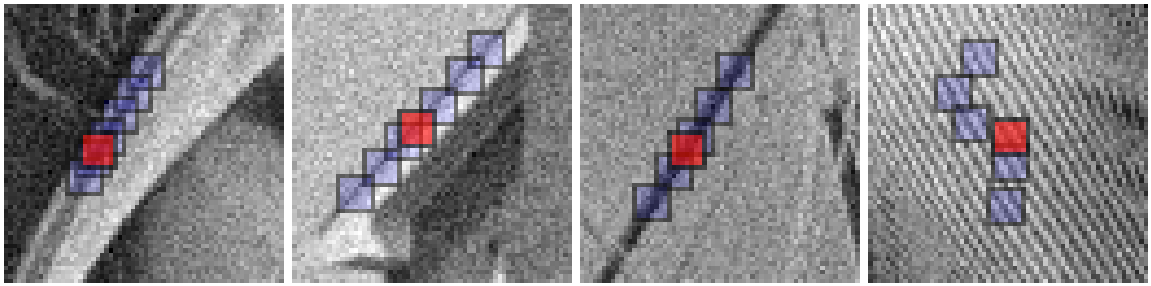
\includegraphics[width=12cm]{bm3d_matching_blocks.png}
 \end{center}
 \caption[The BM3D algorithm.]{The BM3D algorithm. The images show cutaways of {\em Lena}, {\em House}, {\em Boats} and {\em Barbara} images corrupted by zero-mean additive Gaussian noise of $\sigma = 15/255$. A reference block {\em R} and a few of its matched ones illustrate block matching. Taken from \cite{bm3d}.}
 \label{fig:bm3d_example}
\end{figure}

\section{Tico's wavelet method (2009)}
\label{sec:tico09}

Tico presents in \cite{tico09} a relatively simple wavelet-based approach to blurred and noisy image fusion. Input (blurred and noisy) images are first decomposed into their respective wavelet coefficients by using  {\em undecimated} (also known as {\em stationary}) discrete wavelet transformation. Then, multi-level coefficient blending is performed. Finally, inverse wavelet transform is performed yielding the result image.

We observe that the absolute difference between the blurred and noisy images is due to presence of noise in the short-exposed image and blurring in the other. We therefore aim for an estimator that emphasizes the short-exposed image where the absolute difference between the two images is larger, and the long-exposed image otherwise. To achieve better separation between the signal and noise, an image estimator is derived in the wavelet domain. The edge locations (i.e., large values in the difference signal), are emphasized at some scales whereas the noise variance is evenly distributed across the scale space. Considering an orthonormal wavelet transform of the two images, denoting by $G_i(k)$, the $k$-th wavelet coefficient and assuming the same overall brightness of both images\footnote[4]{The same overall brightness for both long and short exposure images can in practice be achieved by proper experimental setup}, we have
%%%
\begin{equation}
	\label{eq:tico09_model}
	\begin{aligned}
		G_1(k) &= F(k) &+ \ N_1(k) \\
		G_2(k) &= F_b(k) &+ \ N_2(k) \\
	\end{aligned}
\end{equation}
%%%
Where $F_b$ denotes the blurred image as a whole since the nature of blurring is not important in this case. Using the observation $\sigma_1^2 \gg \sigma_2^2$ we neglect the noisy coefficients $N_1(k)$ and the term $N_2(k)$ becomes $N(k)$.

We can now fuse the images together using different weights at different scales.  Taking advantage of the de-correlation in the wavelet domain, we propose a minimum mean square error diagonal estimator of the original image in the form of a linear combination between the wavelet coefficients of the two images
%%%
\begin{equation}
\label{eq:tico09_estimator}
	\widehat{F}(k) = G_1(k) + W(k)D(k) \\
\end{equation}
%%%
where $\widehat{F}(k)$ stands for the wavelet coefficients of the restored image, $D(k) = G_2(k) - G_1(k)$ denotes the difference signal between the wavelet coefficients of the two observed images, and $W(k)$ are weight coefficients.  We can estimate the best weight $W(k)$ for each wavelet coefficient by minimizing the mean squared error
%%%
\begin{equation}
\label{eq:tico09_weight}
	E[\|\widehat{F}(k)- F(k)\|]_2^2 = E[\|G_1(k) - F(k) + W(k)D(k)\|]_2^2 \\
\end{equation}
%%%
whose derivative with respect to $W(k)$ equated with zero yields
%%%
\begin{equation}
\label{eq:tico09_weight_derivative}
	W(k)E[\|D(k)\|^2] = E[D(k)N(k)] \\
\end{equation}
%%% 

The computation of the weight $W(k)$ requires an estimate of the noise variance in the short-exposed image, and an estimate of the term $E[\|D(k)\|^2]$.  In order to estimate noise variance in the short-exposed image the approach presented by Mallat in \cite{mall09} where noise variance is calculated by using the median absolute deviation $M_x$\footnote[5]{Median absolute deviation on an univariate sample of quantitative data is defined as $MAD = median_i( | X_i - median_j(X_j)|) $} of the finest-scale wavelet coefficients  as $\sigma \approx M_x/0.6745$ is used. Given the fact that in practice noise is spatially variant over the image, we apply the wavelet-based noise estimate in the pixel neighborhood (e.g. $7x7$). Finally, the $E[\|D(k)\|^2]$ is approximated with $max(\sigma^2(k),avg(|D(k)|^2))$ where $avg$ denotes local spatial average and $\sigma^2(k)$ is the noise variance at the spatial location that corresponds to the $k$-th wavelet coefficient.

As a consequence, the weight $W(k)$ emphasizes the short exposed image in areas of image transitions (edges, for example) whereas the blurred image is emphasized in smooth regions. 

\section{Šroubek and Flusser's method (2003)}
\label{sec:srou03}

Šroubek and Flusser's MCAM algorithm, published in 2003 \cite{srou03}, presents a solution to the SIMO ({\em single input, multiple output}) multichannel blind deconvolution in the presence of noise, which is assumed to be Gaussian of zero mean and variance $\sigma^2$. We extend this algorithm to accomodate noise of different variance per each channel and use it in our 2 channel setting. It has been selected due to its high resilience to noise, no assumptions on the input PSFs and its potential to better accomodate real-life situations, as some amount of blurring typically occurs even in the short-exposed image. 

Expressed mathematically, the algorithm assumes the input to be in the form
%%%
\begin{equation}
\label{eq:srou03_general_model}
	g_i(\mathbf{x}) = f(\mathbf{x}) \star d_i(\mathbf{x}) + n(\mathbf{x}) 	
\end{equation}
%%%
where $g_i$ are observed images, $f$ is the original image, $d_i$ are blur PSFs, $n$ is Gaussian zero-mean noise of variance $\sigma^2$, $i \in \{1 \dots P\}$ is the channel number and $P \subset \mathbb{N}$ is the number of channels. As we can see, this approach is an extension of our model given by formula \ref{eq:general_model}, albeit with the assumption of constant noise in each channel. 

To achieve its task, the algorithm seeks to minimize the energy functional 
%%%
\begin{equation}
\label{eq:srou03_energy}
	E(f, d_1, \dots, d_P) = \frac{1}{2} \sum_{p=1}^{P} || g_p - f \star d_p ||^2 + \lambda Q(f) + \gamma R(d_1, \dots , d_P)	
\end{equation}
%%%
with respect to $f$ and $d_1 \dots d_P$. $Q(f)$ and $R(d_1, \dots, d_P)$ are regularization terms for the original image and blur PSF estimates and $\lambda$ and $\gamma$ are parameters affecting their influence. 

The regularization term $Q(f)$ adopts the total-variation form introduced by Rudin et al. in \cite{rudi92}
%%%
\begin{equation}
\label{eq:srou03_Q_TV}
	Q_{TV}(f) = \int_{\Omega}{} |\nabla f| 	
\end{equation}
%%%
which, compared to other forms of regularization such as Tichonov's $Q_{TV}(f) = \int_{\Omega}{} |\nabla f|^2$ that assume $f$ to be smooth and introduce unwanted ringing artifacts, provides better results. 
The regularization term $R(d_1, \dots, d_P)$ takes the form 
%%%
\begin{equation}
\label{eq:srou03_R}
	R(d_1, \dots, d_P) = \sum_{1 \leq i < j \leq P}^{} || g_i \star d_j - g_j \star d_i ||^2 	
\end{equation}
%%%
Making use of the vector-matrix notation, the $P$-channel acquisition model can be expressed as 
%%%
\begin{equation}
\label{eq:srou03_general_model_vec}
	\mathbf{g} = \mathcal{D}\mathbf{f} + \mathbf{n} = \mathcal{F}\mathbf{d} + \mathbf{n} 	
\end{equation}
%%%
where $\mathbf{f} = [\mathbf{f_1}^T, \dots, \mathbf{f_P}^T]^T$ and $\mathbf{d} = [\mathbf{d_1}^T, \dots, \mathbf{d_P}^T]^T$ are aggregate vector forms of $f$ and $d$. The matrices $\mathcal{D}$ and $\mathcal{F}$ are defined as 
%%%
\begin{equation}
\label{eq:srou03_general_model_vec}
	\mathcal{F} \equiv \begin{pmatrix} \mathbf{F} & \cdots & 0 \\ \vdots & \ddots & \vdots \\ 0 & \cdots & \mathbf{F} \end{pmatrix} \text{ and } \mathcal{D} \equiv \begin{pmatrix} \mathbf{D_1} \\ \vdots \\ \mathbf{D_P} \end{pmatrix}  	
\end{equation}
%%%
where $\mathbf{F}$ and $\mathbf{D_i}$ are vector-matrix forms of $f$ and $d_i$. The modified energy functional then assumes the form
%%%
\begin{equation}
\label{eq:srou03_energy_vec}
	E(\mathbf{d},\mathbf{f}) = \frac{1}{2}||\mathcal{D}\mathbf{f} - \mathbf{g}||^2 + \lambda  \mathbf{f}^T \mathcal{L} \mathbf{f} + \gamma ||\mathcal{Z} \mathbf{d}||^2 	
\end{equation}
%%%   
Here, the use of $\mathcal{L}$ matrix achieves the computation of total variance from equation \ref{eq:srou03_Q_TV} in discrete form. The matrix $\mathcal{Z}$ achieves the same goal for the computation of regularization term in equation \ref{eq:srou03_R}. 
Expanding the terms $\frac{1}{2}||\mathcal{D}\mathbf{f} - \mathbf{g}||^2$ (which is equivalent to $\frac{1}{2}||\mathcal{F}\mathbf{d} - \mathbf{g}||^2$) and $||\mathcal{Z} \mathbf{d}||^2$ yields the energy functional in the form
%%%
\begin{equation}
\label{eq:srou03_energy_vec_exp}
	E(\mathbf{d},\mathbf{f}) = \frac{1}{2}[\mathbf{d}^T \mathcal{F}^T \mathcal{F} \mathbf{d}  - 2 \mathbf{g}^T \mathcal{F} \mathbf{d} + \mathbf{g}^T \mathbf{g}] + \lambda \mathbf{f}^T \mathcal{L} \mathbf{f} + \gamma \mathbf{d}^T \mathcal{Z}^T \mathcal{Z} \mathbf{d}	
\end{equation}
%%%
To obtain solutions for the minimal $\mathbf{d}$ and $\mathbf{f}$, we solve the system of differential equations
%%%
\begin{equation}
\label{eq:srou03_energy_vec_partial}
	\begin{aligned}
		\frac{\partial E(\mathbf{d},\mathbf{f})}{\partial \mathbf{d}} &= 2 \mathcal{F}^T \mathcal{F} \mathbf{d} &- \ 2 \mathcal{F}^T \mathbf{g} &+ 2 \gamma \mathcal{Z}^T \mathcal{Z} \mathbf{d} &= 0 \\	
		\frac{\partial E(\mathbf{d},\mathbf{f})}{\partial \mathbf{f}} &= 2 \mathcal{D}^T \mathcal{D} \mathbf{f} &- \ 2 \mathcal{D}^T \mathbf{g} &+ 2 \lambda              \mathcal{L} \mathbf{f} &= 0
	\end{aligned}
\end{equation}
%%%
from which we obtain the expressions for the solutions of $\mathbf{d}$ and $\mathbf{f}$
%%%
\begin{equation}
\label{eq:srou03_solutions}
	\begin{aligned}
		( &\mathcal{F}^T \mathcal{F} &+ \ \gamma \mathcal{Z}^T \mathcal{Z} ) \mathbf{d} &= \mathcal{F}^T \mathbf{g} \\
		( &\mathcal{D}^T \mathcal{D} &+ \ \lambda              \mathcal{L} ) \mathbf{f} &= \mathcal{D}^T \mathbf{g}	
	\end{aligned}
\end{equation}
%%% 
and finally we obtain the values of $\mathbf{f}$ and $\mathbf{d}$ through the alternating minimization algorithm, which consists of the following steps.
%%%
\begin{algorithmic}
	\REQUIRE Initial value $\mathbf{f}^0$, blur size $(m_d, n_d)$ and regularization parameters $\gamma$, $\lambda$
	\FOR{$n \geq 1$} 
		\STATE $\mathbf{d}^n \gets$ solve $[(\mathcal{F}^{n - 1})^T \mathcal{F}^{n - 1} + \gamma \mathcal{Z}^T \mathcal{Z} ] \mathbf{d}^n = (\mathcal{F}^{n - 1})^T \mathbf{g}$ 
		\STATE set $\mathbf{h}^0 = \mathbf{f}^{n - 1}$ and $v^0 = \phi(\mathbf{f}^{n - 1})$ 
		\FOR{$k \geq 1$}
			\STATE $\mathbf{f}^k \gets$ solve $[(\mathcal{D}^n)^T \mathcal{D}^n + \lambda \mathcal{L} v^{k-1} ] \mathbf{f}^k = (\mathcal{D}^n)^T \mathbf{g}$
			\STATE $v^k = \phi(\mathbf{h}^k)$
		\ENDFOR
		\STATE $\mathbf{f}^n \gets \mathbf{h}^k$
	\ENDFOR
\end{algorithmic}

The $\phi$ function in the inner loop $k$ serves as an auxiliary function introduced to solve the minimization of $Q(u)$ as $\partial Q(u) / \partial u$ is a highly nonlinear function which is not defined for $|\nabla u| = 0$. 

Parameters $\gamma$ and $\lambda$ providing the best results are usually obtained empirically, but can be estimated from equation \ref{eq:srou03_solutions} to obtain better starting values. Under the $\mathbb{L}_2$ norm, we obtain
%%%
\begin{equation}
\label{eq:srou03_gamma_lambda}
	\begin{aligned}
		\gamma^2  &= \frac{ ||\mathcal{F}^\mathcal{T}(\mathcal{F} \mathbf{d} - \mathbf{g}) ||^2 }{ || \mathcal{Z}^T \mathcal{Z} \mathbf{d} ||^2} \\
		\lambda^2 &= \frac{ ||\mathcal{D}^\mathcal{T}(\mathcal{D} \mathbf{f} - \mathbf{g}) ||^2 }{ || \mathcal{L}   \mathbf {f} ||^2}   	
	\end{aligned}
\end{equation}
%%%
Since $F \mathbf{d} - \mathbf{g} = D \mathbf{f} - \mathbf{g}$ is equal to white Gaussian noise $\mathbf{n}$ and $||\mathbf{n}||^2 \approx P m_f n_f \sigma^2$, it is easy to observe from the properties of vector-matrix notation that $||\mathcal{F}^T(\mathcal{F} \mathbf{d} - \mathbf{g}) ||^2 \approx P m_d n_d ||\mathbf{f}||^2 \sigma^2$. Given the fact that $\mathbf{d}$ stands for the correct PSFs, it must be a linear combination of $\mathcal{Z}^T \mathcal{Z} $ eigenvectors that correspond to a set of minimal eigenvalues, which can be expressed as $||\mathcal{Z}^T \mathcal{Z} \mathbf{d}||^2 = \lambda_1^2 ||\mathbf{d}||^2$. From the definition of $\mathcal{Z}$ it follows that $\lambda_1 \approx \sigma^2 (P-1) m_f n_f$, yielding the final form of approximation 
%%%
\begin{equation}
\label{eq:srou03_gamma_estimate}
	|\gamma| = \frac{1}{P - 1} \frac{\sqrt{P m_d n_d}}{|| \mathbf{d} ||} \frac{||\mathbf{f}||}{m_f n_f} \frac{1}{\sigma}
\end{equation}
%%%
The $\mathbb{L}^2$ norms of $\mathbf{f}$ and $\mathbf{d}$ are not known in advance, but the former can be approximated by $\mathbf{g}$ and the latter, given that elements in each PSF must sum up to 1, is bound within $(P / (m_d n_d)^2) \leq || \mathbf{d} ||^2 \leq 1$. 

A similar procedure is applied to the estimate of the $\lambda$ parameter, but only a bottom limit can be obtained. The uncertainty resides in the term $||\mathcal{L} \mathbf{f}||^2$ which cannot be further simplified since it is completely dependent on the local behavior of $f$. The bottom limit in general is zero; the upper limit can be generously defined as $||\mathcal{L} \mathbf{f}||^2 \leq c^2 ||\mathbf{f}||^2$. The $c$ constant is dependent on the used regularization term, that is $c = 4$ for the $\mathcal{L}_4$ and $c = 4 + 4(1/\sqrt{2})$ for the $\mathcal{L}_8$ TV. Given the fact that $||\mathcal{D}^T (\mathcal{D} \mathbf{f} - \mathbf{g}) ||^2 \approx || \mathbf{d} ||^2 \sigma^2 m_f n_f$, the bottom limit is expressed as
%%%
\begin{equation}
\label{eq:srou03_lambda_estimate}
	|\lambda| \gtrapprox \frac{||\mathbf{d}||\sigma}{c} \frac{\sqrt{m_f n_f}}{||\mathbf{f}||}
\end{equation}
%%%

The product of the parameters 
%%%
\begin{equation}
\label{eq:srou03_lambda_estimate}
	|\gamma| |\lambda| \geq \frac{1}{c(P-1)} \sqrt{\frac{P m_d n_d}{m_f n_f}}
\end{equation}
%%%
only depends on the dimension of the problem and establishes a fixed relation between them.


\subsection{Algorithm extension}
\label{sec:srou03_extension}
We propose and implement an extension to the MC-AM algorithm to allow for variable amount of noise in each channel. We assume each channel $i \in {1 \dots P}$ to be corrupted by zero mean white Gaussian noise of variance $\sigma_i^2$, in other words
%%%
\begin{equation}
\label{eq:srou03_general_model_ext}
	g_i(\mathbf{x}) = f(\mathbf{x}) \star d_i(\mathbf{x}) + n_i(\mathbf{x}) 	
\end{equation}
%%%

To achieve this task, we need to balance the contribution of each channel to the overall minimization process. To this end, we need to analyze and assess the influence of variable noise on each of the terms in the energy fuctional described by equation \ref{eq:srou03_energy} and modify it accordingly. 

The first term  
%%%
\begin{equation}
\label{eq:srou03_term_1_ext}
	\sum_{p=1}^{P} || g_p - f \star d_p ||^2 	
\end{equation}
%%%
can be expanded as 
%%%
\begin{equation}
\label{eq:srou03_term_1_ext_exp}
	\sum_{p=1}^{P} || g_p - f \star d_p ||^2 = ||n_1||^2 + ||n_2||^2 + \dots + ||n_P||^2 \approx m_f n_f \sigma_1^2 + m_f n_f \sigma_2^2 + \dots + m_f n_f \sigma_P^2 	
\end{equation}
%%%
from which we can directly observe that each term needs to be multiplied by $\sigma_p^{-2}$ to balance its contribution, we thus obtain
%%%
\begin{equation}
\label{eq:srou03_term_1_ext}
	\sum_{p=1}^{P} \frac{|| g_p - f \star d_p ||^2}{\sigma_p^2} 	
\end{equation}
%%%
as the modification of the first term.

The second, total variation term will not be modified as it is a function of the original image $f$. Its initial value for the algorithm is provided by $g_i$ as is the case in the unmodified version.
It is however important to note that the value of the parameter $\lambda$ will change as a result of our modification, as will be described below. 

The third, blur PSF regularization term $R(d_1 \dots d_P)$ is a sum of terms $|| g_i \star d_j - g_j \star d_i ||^2$, where $1 \leq i < j \leq P$. Each term can be expanded as 
%%%
\begin{equation}
\label{eq:srou03_R_exp}
\begin{split}
	|| g_i \star d_j - g_j \star d_i ||^2 &= || (f \star d_i + n_i) \star d_j - (f \star d_j + n_j) \star d_i ||^2 \\ &=  ||f \star d_i \star d_j - f \star d_j \star d_i +  n_i \star d_j - n_j \star d_i||^2 \\ &= ||n_i \star d_j - n_j \star d_i||^2. 	
\end{split}
\end{equation}
%%%
The term $||n_i \star d_j - n_j \star d_i||^2$ can be simplified further. When we think of convolution, we can visualize it as $\alpha$-blending of $m_d n_d$ shifted copies of the original image, where $\sum{}{} \alpha_i = 1$. Doing the same with noise results also in noise with approximately the same characteristics. We can therefore write
%%%
\begin{equation}
\label{eq:srou03_R_exp_noise}
	||n_i \star d_j - n_j \star d_i||^2 \approx ||n_i - n_j||^2 
\end{equation}
%%%
Since terms $n_i$ and $n_j$ represent uncorrelated noise and $||\dots||^2 = (\dots)^T(\dots)$, we obtain
%%%
\begin{equation}
\label{eq:srou03_R_exp_noise_approx}
\begin{split}
	||n_i - n_j||^2 &= (n_i - n_j)^T(n_i - n_j) \\ &= n_i^T n_i - n_j^T n_i - n_i^T n_j + n_j^T n_j \\ &= n_i^T n_i + n_j^T n_j \\ &\approx m_f n_f (\sigma_i^2 + \sigma_j^2).
\end{split}
\end{equation}
%%%
The regularization term $R(d_1 \dots d_P)$ thus assumes the form
%%%
\begin{equation}
\label{eq:srou03_R_ext}
	R(d_1, \dots, d_P) = \sum_{1 \leq i < j \leq P}^{} \frac{1}{\sigma_i^2 + \sigma_j^2} || g_i \star d_j - g_j \star d_i ||^2 
\end{equation}
%%%

In discrete form, weights are introduced into the first term by matrix multiplication using a block diagonal matrix $\Sigma$ that consists of $P^2$ blocks of size $m_d n_d$. All blocks contain zeros except for the diagonal ones ($\Sigma_{ii}$), which are themselves diagonal matrices containing inverse values of noise standard deviations $\sigma_i^{-1}$. 
%%%
\begin{equation}
\label{eq:srou03_R_ext}
	\left|\left| \begin{pmatrix} \Sigma_1^{-1} & \hdots & 0 \\ \vdots & \ddots & \vdots \\ 0 & \hdots & \Sigma_P^{-1} \end{pmatrix} \left[ \begin{pmatrix} \mathbf{F} & \hdots & 0 \\ \vdots & \ddots & \vdots \\ 0 & \hdots & \mathbf{F} \end{pmatrix}  \begin{pmatrix} \mathbf{d_1} \\ \hdots \\ \mathbf{d_P} \end{pmatrix} - \begin{pmatrix} \mathbf{g_1} \\ \hdots \\ \mathbf{g_P} \end{pmatrix} \right] \right|\right|^2\text{.} 
\end{equation}
%%%
Rather than altering the matrix $\mathcal{Z}$ which is never used directly, we modify the matrix product $\mathcal{Z}^T\mathcal{Z}$. This consists of $P^2$ square blocks of size $m_d n_d$ and is re-defined as follows:
%%%
\begin{equation}
\label{eq:srou03_R_ext}
	\mathcal{Z}^T\mathcal{Z} = ( \mathcal{Z}_{ij} ) = 
	\begin{cases} 
		\frac{1}{\sigma_i^2 + \sigma_j^2}\mathbf{G}_j^T\mathbf{G}_i^{}, & i \neq j \\ 
		\sum_{k \neq i}^{}\frac{1}{\sigma_i^2 + \sigma_k^2}\mathbf{G}_k^T\mathbf{G}_k^{}, & i = j  
	\end{cases}
	\end{equation}
%%%

It is necessary to determine how our modification will affect the estimation of $\gamma$ and $\lambda$ parameters. We can easily observe that the introduction of the $\Sigma$ weight matrix will 
modify the numerator in both $\gamma^2$ and $\lambda^2$ estimation (see equation \ref{eq:srou03_gamma_lambda}) as $||\mathcal{F}^T \Sigma^T \Sigma( \mathcal{F} \mathbf{d} - \mathbf{g}) ||^2$ and $||\mathcal{D}^T \Sigma^T \Sigma( \mathcal{D} \mathbf{f} - \mathbf{g}) ||^2$, respectively. Since 
%%%
\begin{equation}
\label{eq:srou03_lambda_numer}
	||\mathcal{F}^T(\mathcal{F} \mathbf{d} - \mathbf{g}) ||^2 \approx P m_d n_d ||\mathbf{f}||^2 \sigma^2
\end{equation}
%%%
and 
%%%
\begin{equation}
\label{eq:srou03_gamma_numer}
	||\mathcal{D}^T (\mathcal{D} \mathbf{f} - \mathbf{g}) ||^2 \approx || \mathbf{d} ||^2 \sigma^2 m_f n_f
\end{equation}
%%%
and $\sigma_i^{-2}$ emerge from the $\mathbb{L}_2$ norm as $\sigma_i^{-4}$, we obtain the modified numerators in the form    
%%%
\begin{equation}
\label{eq:srou03_lambda_numer_ext}
	||\mathcal{F}^T(\mathcal{F} \mathbf{d} - \mathbf{g}) ||^2 \approx m_d n_d ||\mathbf{f}||^2 \sum_{i=1}^{P} \frac{1}{\sigma_i^2} 
\end{equation}
%%%
and 
%%%
\begin{equation}
\label{eq:srou03_gamma_numer_ext}
	||\mathcal{D}^T (\mathcal{D} \mathbf{f} - \mathbf{g}) ||^2 \approx  m_f n_f \sum_{i=1}^P \frac {|| \mathbf{d}_i ||^2}{ \sigma_i^2}
\end{equation}
%%%
The denominator $|| \mathcal{L} \mathbf{f} ||^2$ in the $\lambda^2$ estimation equation remains unaffected. To evaluate the change in the $|| \mathcal{Z}^T \mathcal{Z} \mathbf{d} ||^2$ denominator, let us first assume that each of the $P$ channels is corrupted by Gaussian zero-mean noise of the same variance $\sigma^2$. This will, according to our modification of the $\mathcal{Z}^T \mathcal{Z}$ matrix in equation \ref{eq:srou03_R_ext}, lead to a matrix in which each element is multiplied by $1/2\sigma^2$. Thus, in this special case, we obtain the modified $\mathcal{Z}^T \mathcal{Z}$ matrix simply by multiplying the original by $1/2\sigma^2$. Under the $L_2$ norm, this term will cancel out the $\sigma^2$ from the above estimation of eigenvalue $\lambda_1$, yielding the final form of the gamma estimate
%%%
\begin{equation}
\label{eq:srou03_gamma_estimate_ext}
	|\gamma| = \frac{2}{P - 1} \sqrt{ \frac{m_d n_d}{|| \mathbf{d} ||^2} \frac{||\mathbf{f}||^2}{m_f^2 n_f^2} \sum_{i=1}^{P} \frac{1}{\sigma_i^2} }
\end{equation}
%%%
and of the lambda estimate
%%%
\begin{equation}
\label{eq:srou03_lambda_estimate_ext}
	|\lambda| \gtrapprox \frac{1}{c} \sqrt{ \frac{m_f n_f}{||\mathbf{f}||^2} \sum_{i=1}^{P}\frac{||\mathbf{d}_i||^2}{\sigma_i^2}}
\end{equation}
%%%
We use the theoretically computed values of $\gamma$ and $\lambda$ in experiments for both simulated and real-world data.  

\chapter{Results}
\label{chap:results}

In this chapter, we present the results of tests that have been performed on both simulated and real-world data. We begin by describing the experimental setup used to obtain the data in section \ref{sec:experimental_setup}. This is followed by a separate presentation of results for simulated and real-world data in sections \ref{sec:simulated_data} and \ref{sec:real_world_data}, respectively. The chapter concludes with an analysis and discussion of our findings in section \ref{sec:evaluation}.

\clearpage

\section{Experimental setup}
\label{sec:experimental_setup}

\subsection{Setup for simulated data}
\label{sec:setup_for_simulated_data}

We have used a set of 4 point spread functions (see figure \ref{fig:used_psfs}) and 4 testing images (see figure \ref{fig:used_psfs}). These were selected in order to reflect various environments and conditions in which taking images could take place. 
%%%
\begin{figure}[htb]
 \begin{center}
  
\includegraphics[width=12cm]{used_psfs.png}
 \end{center}
 \caption{Point-spread functions selected for use in testing.}
 \label{fig:used_psfs}
\end{figure}
%%%
\begin{figure}[htb]
 \begin{center}
  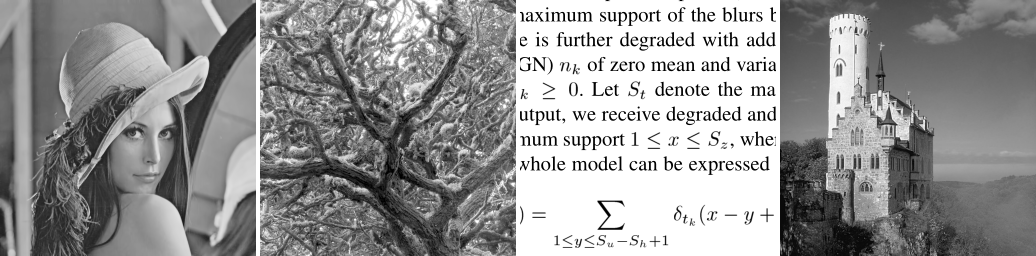
\includegraphics[width=12cm]{used_images.png}
 \end{center}
 \caption{Images selected for use in testing.}
 \label{fig:used_images}
\end{figure}

Testing images used were 256 by 256 pixels in size. We avoided the use of larger resolutions since they tend to be computationally expensive, especially in case of Šroubek's algorithm. The PSF sizes were $2^n - 1$, with $n$ being an integer in range $\lbrace 2 \dots 5 \rbrace$. Odd-sized PSFs are preferred due to the fact that they have a well-defined center. The range of used PSF sizes corresponds to results attained in real-world experiments which, altough greatly dependent on the individual photographer's steadiness while taking pictures,  did not exceed 31 pixels. This is described in section \ref{sec:real_world_data}. We've performed experiments for both simulated ISOs (the ``ISO mode'') and additive white Gaussian noise  (the ``variance mode'').

Since Ojala in \cite{ojal08} demonstrated that temperature and exposure time have very little influence on the level of noise present in a digital photograph, we chose to abandon these parameters completely, leaving ISO as the only parameter. ISO 100 was chosen as the base value for both generated and real-world data. 

In case of generated data, the pair of ISO values is chosen in advance, one of the values being 100 for the blurred, less noisy image. The other value is set to $100*2^i$, where $i$ is an integer greater than 1. This corresponds to ISO settings usually present in digital cameras; however, as of 2011, ISO settings over 25600 are rarely encountered in commercially available products, requiring us to use a value of $i$ no greater than 8. We have, however, also used the $i$ value of 10 (ISO 102400) to generate noise which cannot be simply approximated as a zero-mean Gaussian and thus pose potential difficulty for the BM3D denoising algorithm.  

Fixing the low ISO value at 100, the choice of the high ISO value depends on the level of illumination we wish to emulate. The lower the amount of light in the photographed scene, the higher ISO we need to compensate for the potentially longer exposure time (and thus larger blurring) needed for the camera to capture enough light. For example, given a 2 second exposure time to achieve a proper level of lighting at ISO 100, we might even need to go to ISO 12800 to achieve a potentially blur-less exposure at $1/60$ seconds. To achieve approximately the same level of illumination in both short and long exposure images, their ISO and shutter speed settings need to satisfy the equation $ISO_s t_s = ISO_l t_l$. Dynamic ranges of images taken in real-world experiments have confirmed this rule with a sufficient degree of precision.  

In total, we've used 4 different images, 4 different blur PSFs at 4 different sizes and 9 different ISO settings, totalling 576 testing scenarios. 

For each experiment, the input is a tuple ({\em input image}, {\em input PSF}, {\em input PSF size}, {\em noisy image ISO}). The ISO value for the blurred image is fixed at 100. We first read the input image, create two copies, one of which is subject to ISO simulation at the {\em noisy ISO} value, the other is blurred using the {\em input PSF} resized to {\em input PSF size} and subject to ISO simulation at ISO 100. In the next step, noise standard deviation is estimated from both noisy and blurred image as the standard deviation of the difference between the noisy and the original image and blurred and noisy and blurred and noiseless image, respectively. We proceed to remove noise from the noisy image using the BM3D algorithm using the estimated noise variance and to execute both Šroubek's and Tico's algorithms on the blurred - noisy image pair. The noisy and blurred images and the images resulting from the three other methods are written into separate files, as is the initial estimate of the blur PSF and the resulting blur PSFs from Šroubek's algorithm. We then compute signal to noise ratios from all images. A record of each experiment is also written to an output *.csv file. The record features the name of the image and PSF used, the PSF size, the ISO value used for blurred and noisy image, the values of estimated noise standard deviations, the $\lambda$ and $\gamma$ parameters used by Šroubek's algorithm and signal-to-noise ratios for the blurred, noisy and other resulting images.  

As we've mentioned earlier, we had also performed experiments using the same images and blur PSFs in variance mode, where the images were corrupted by additive white Gaussian noise of variances $10^{-i}$, $i$ being in range $\lbrace 1 \dots 4 \rbrace$. The base image was corrupted by additive white Gaussian noise of variance $10^{-5}$. Again, there were 4 input images, 4 different blur PSFs at 4 different sizes and 4 noise levels, bringing the total to 256 experiments. Similarly to the ISO mode, the input of each experiment is a tuple ({\em input image}, {\em input PSF}, {\em input PSF size}, {\em noisy image variance}) and noise variance of the blurred (base) image is fixed at $10^{-5}$. We do not need to estimate noise standard deviation in any of the images as it is already given. The format of output files and the record written to *.csv file differs only in ISO being replaced by noise variance and the estimates of noise standard deviation not being present at all. 

The resulting *.csv report files are then processed to obtain useful data. The images and *.csv records from all experiments are included on the CD in their entirety.

\subsection{Setup for real-world data}
\label{sec:setup_for_real_world_data}

Real-world experiments were performed by projecting the Lena image on a vertical white wall $2.6$ by $2.6$ metres in size and taking images of it with a Canon EOS 5D digital SLR camera using an $85$ mm lens at a distance of $5$ meters. The projector's optical axis was not perpendicular to the projecting wall; however, a dedicated setting of the projector was used to compensate. The projected image was $70$ by $70$ centimeters in size and was carefully measured vertically, horizontally and diagonally to rule out any spatial distortion.  Sources of light other than the projector itself were blocked out to prevent light pollution and color interference. Control over the level of illumination was achieved by multiplying the image function by a constant; $0.5$, $0.25$ and $0.125$ were the values used (the resulting images were too bright for multiplier $1$ - the original Lena image). Since the projector's output resolution was $800$ by $600$ pixels and the used image was $256$ by $256$ pixels in size, it was possible to insert control features (pixels and crosses) in the otherwise unused part of the projected space (see \ref{fig:testing_image_control_points}). These features were used to align the obtained images and to directly observe PSF shapes. 
%%%
\begin{figure}[htb]
 \begin{center}
  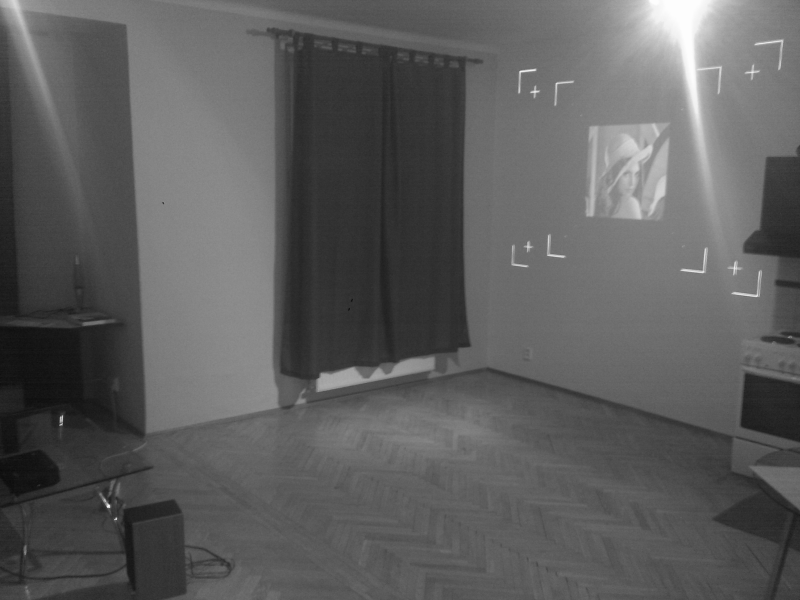
\includegraphics[width=12cm]{testing_setup.png}
 \end{center}
 \caption{Setup for real-world testing.}
 \label{fig:testing_setup}
\end{figure}
%%%
\begin{figure}[htb]
 \begin{center}
  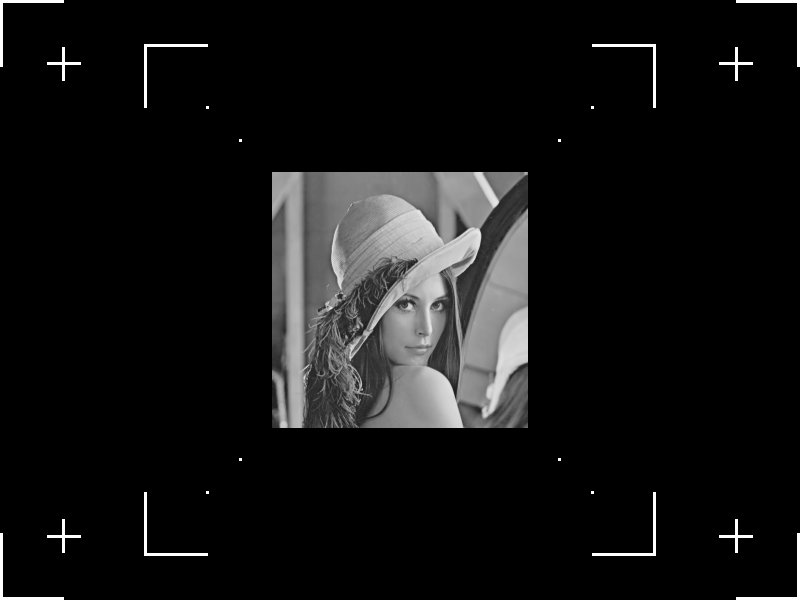
\includegraphics[width=12cm]{testing_image_control_points.png}
 \end{center}
 \caption{An example of a testing image with control features.}
 \label{fig:testing_image_control_points}
\end{figure}
%%%

Three experiments were carried out, one for each multiplier value. In each experiment, several (about $20$) images were taken at a progressively greater camera ISO setting until the images produced contained little or no blurring. All images were taken in aperture priority mode with aperture set to the lowest possible value, $1.8$. For each experiment, a set of two images was selected; the first taken with ISO set to $100$ (the blurred image) and the second taken at the lowest ISO setting that produced little or no blurring (the ``noisy'' images). These images were processed as follows: 

%%%
\begin{enumerate}
\item Images are converted from $24$ bits per pixel color JPEG to $8$ bits per pixel PNG.
\item Images are semi-manually registered in Matlab using the \texttt{cpselect}, \texttt{cp2tform} and \texttt{imtransform} routines. The registration process (see figure \ref{fig:registration_process}) also downsamples the images from their original $4368$ by $2912$ pixels resolution to less than $800$ by $600$ needed for further processing. 
\item Registered images are manually aligned (Paint.NET image editor was used). Figure \ref{fig:alignment_process} illustrates the result of one such alignment.
\item PSF size for the blurred image is determined by fitting the blur kernel in the smallest possible odd-sized square region with a small margin.
\item A region of the same size as the input image is cut from the blurred and noisy image in their aligned position.
%%\item Blurred and noisy images obtained by cropping in the previous step have their statistics (mean and standard deviation) matched with the original Lena image using the color transfer method by Reinhard et al.\cite{rein01}
\item Noise standard deviation is estimated from both images as an average value of the results of the 4 available methods (see section \ref{sec:estimation_of_noise_from_images}).
\item The noisy image is denoised by the BM3D algorithm using the estimated noise standard deviation value.
\item The noisy and blurred images are subject to Tico's wavelet fusion and Šroubek's MC-AM deconvolution.
\item Resulting images are evaluated in terms of SNR and visual quality.
\end{enumerate}
%%%

%%%
\begin{figure}[htb]
 \begin{center}
  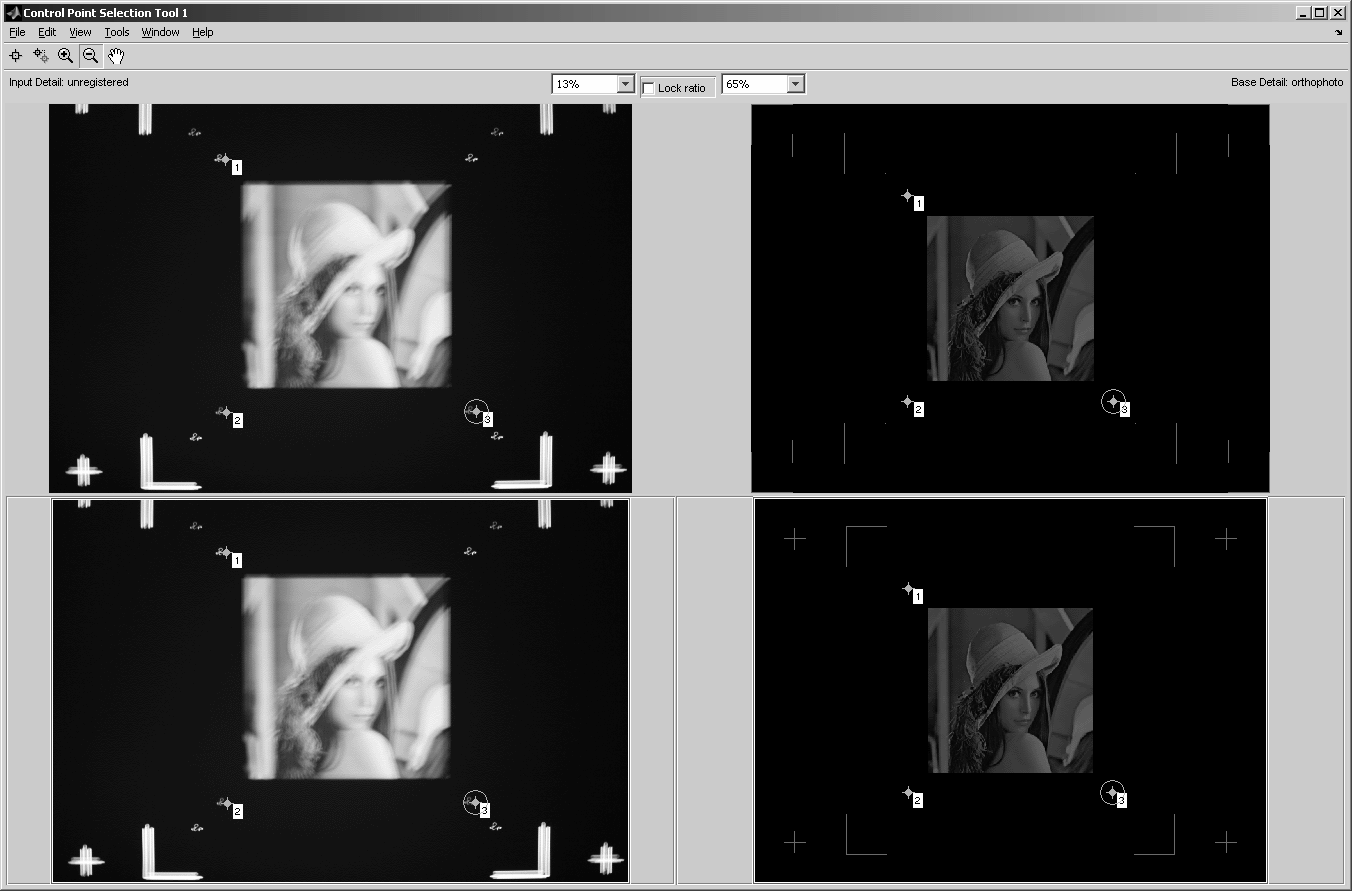
\includegraphics[width=12cm]{registration_process.png}
 \end{center}
 \caption{Image registration process in Matlab, feature point selection.}
 \label{fig:registration_process}
\end{figure}
%%%

%%%
\begin{figure}[htb]
 \begin{center}
  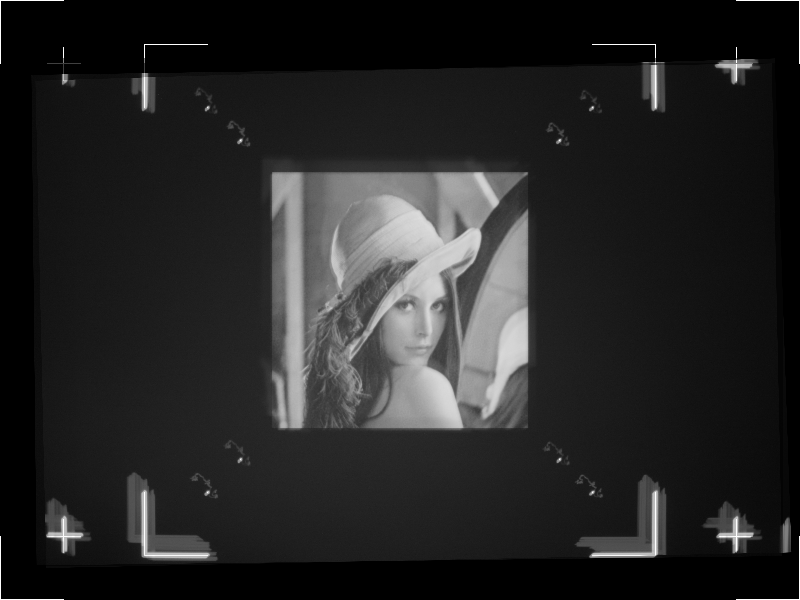
\includegraphics[width=12cm]{alignment_process.png}
 \end{center}
 \caption{The result of image alignment for experiment 1.}
 \label{fig:alignment_process}
\end{figure}
%%%


\section{Results for simulated data}
\label{sec:simulated_data}

From the total of $576$ experiments performed in ISO mode, our modification of the Šroubek's algorithm provided the best results in terms of SNR in 182 cases. Of those 182 cases, 122 were marked with a difference greater than 1 dB from the result of the BM3D algorithm, which provided the best result in 393 cases (277 of which with a difference greater than 1 dB from the result of Šroubek's algorithm). Tico's algorithm provided the best result in a single case (Lena image, diagonal-line shaped PSF of size 3 for the blurred image and ISO 102400 for the noisy image), which is illustrated by figure \ref{fig:tico09_iso_success}.  The SNR of Tico's result was 14.2735 compared to Šroubek's 13.813 and 13.7881 for the BM3D algorithm.

Of the total of $256$ experiments performed in variance mode, Šroubek's algorithm provided the best results in terms of SNR in 126 (88) cases, the BM3D was more successful in 128 (85) cases and Tico's algorithm in 2. The relatively higher success rate of Šroubek's algorithm can be explained by lower performance of the BM3D algorithm in extremely noisy conditions (variances 0.01 and 0.1) which were not achieved by ISO simulation. In comparison, the simulated ISO of 25600 corresponds to AWGN variance of about 0.003 for all images, the extreme simulated ISO value of 102400, which is only encountered in high end digital SLRs, corresponds to AWGN\footnote[6]{Additive white Gaussian noise.} variance of about 0.02, which is still an order of magnitude less than the highest value used in variance mode. 

Both of the two marginally successful results of Tico's algorithm in variance mode were achieved in conditions of extreme noise in the noisy image (variance 0.1) and extreme blurring in the other (PSF sizes 15 and 31), one of which is illustrated by figure \ref{fig:tico09_var_success}. The SNR of Tico's result was 5.3947 compared to Šroubek's 2.5659 and 5.0676 for the BM3D algorithm. 


\begin{figure}[htb]
 \begin{center}
  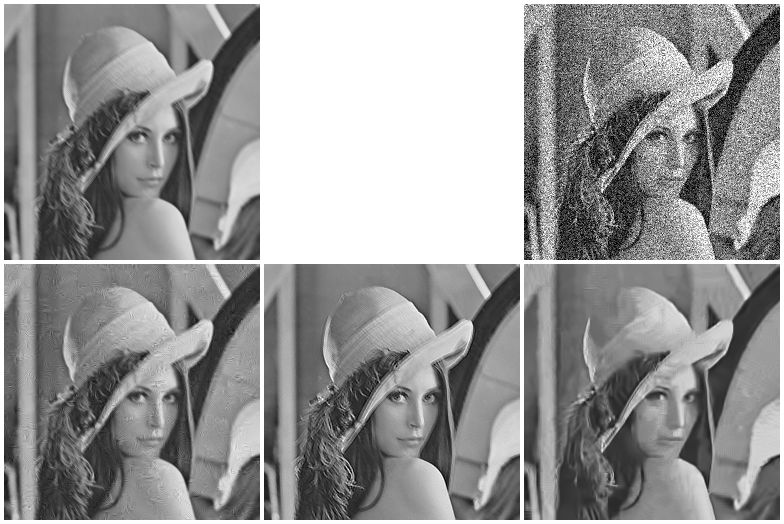
\includegraphics[width=12cm]{tico09_iso_success.png}
 \end{center}
 \caption{Top row: the blurred and noisy image pair for the successful result of the Tico's algorithm in ISO mode. Bottom row: the results of Tico's and Šroubek's methods and the BM3D algorithm.}
 \label{fig:tico09_iso_success}
\end{figure}

% subfloat version
\begin{figure}[htb]
  \begin{center}
	  \subfloat[]{\label{fig:tico09_iso_success_blurred}
\includegraphics[width=0.3\textwidth]{tico09_iso_success_blurred.png}}
	  ~
	  \subfloat[]{\label{fig:tico09_iso_success_psfs}
\includegraphics[width=0.3\textwidth]{tico09_iso_success_psfs.png}}
	  ~
	  \subfloat[]{\label{fig:tico09_iso_success_noisy}
\includegraphics[width=0.3\textwidth]{tico09_iso_success_noisy.png}}

	  \subfloat[]{\label{fig:tico09_iso_success_tico09}
\includegraphics[width=0.3\textwidth]{tico09_iso_success_tico09.png}}
	  ~
	  \subfloat[]{\label{fig:tico09_iso_success_srou03}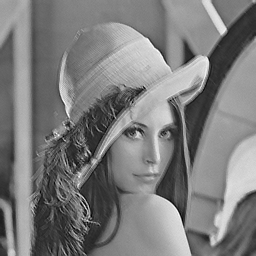
\includegraphics[width=0.3\textwidth]{tico09_iso_success_srou03.png}}
	  ~
	  \subfloat[]{\label{fig:tico09_iso_success_bm3d}
\includegraphics[width=0.3\textwidth]{tico09_iso_success_bm3d.png}}
  \caption[The successful result of the Tico's algorithm in ISO mode.]{The successful result of the Tico's algorithm in ISO mode. Top row: the blurred and noisy image pair for the successful result of the Tico's algorithm in ISO mode. Bottom row: the results of Tico's and Šroubek's methods and the BM3D algorithm.}
  \end{center}
  \label{fig:tico09_iso_success}
\end{figure}



\begin{figure}[htb]
 \begin{center}
  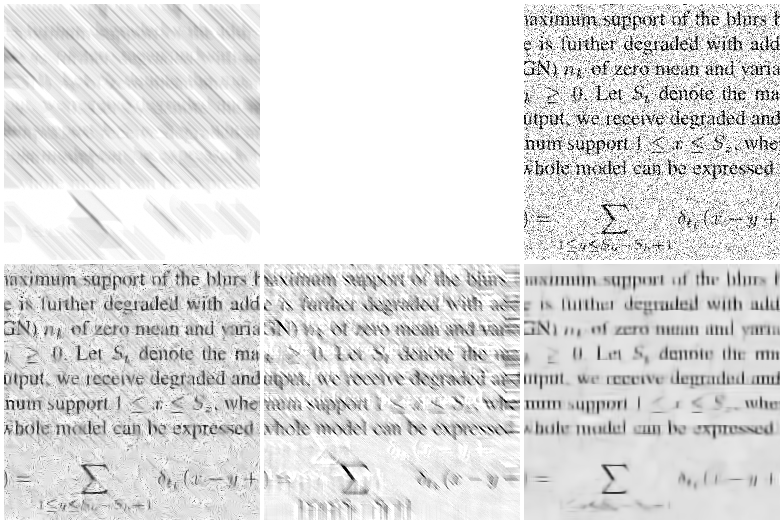
\includegraphics[width=12cm]{tico09_var_success.png}
 \end{center}
 \caption{Top row: the blurred and noisy image pair for the successful result of the Tico's algorithm in variance mode. Bottom row: the results of Tico's and Šroubek's methods and the BM3D algorithm.}
 \label{fig:tico09_var_success}
\end{figure}

%% subfloat version
\begin{figure}[htb]
  \begin{center}
	  \subfloat[]{\label{fig:tico09_var_success_blurred}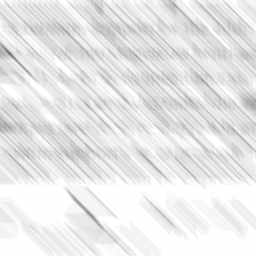
\includegraphics[width=0.3\textwidth]{tico09_var_success_blurred.png}}
	  ~
	  \subfloat[]{\label{fig:tico09_var_success_psfs}
\includegraphics[width=0.3\textwidth]{tico09_var_success_psfs.png}}
	  ~
	  \subfloat[]{\label{fig:tico09_var_success_noisy}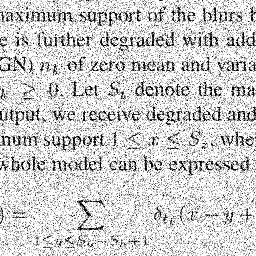
\includegraphics[width=0.3\textwidth]{tico09_var_success_noisy.png}}

	  \subfloat[]{\label{fig:tico09_var_success_tico09}
\includegraphics[width=0.3\textwidth]{tico09_var_success_tico09.png}}
	  ~
	  \subfloat[]{\label{fig:tico09_var_success_srou03}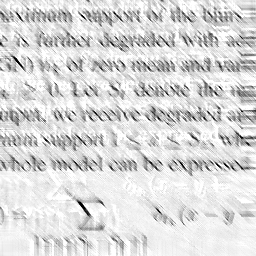
\includegraphics[width=0.3\textwidth]{tico09_var_success_srou03.png}}
	  ~
	  \subfloat[]{\label{fig:tico09_var_success_bm3d}
\includegraphics[width=0.3\textwidth]{tico09_var_success_bm3d.png}}
  \caption[The successful result of the Tico's algorithm in variance mode.]{The successful result of the Tico's algorithm in variance mode. Top row: the blurred and noisy image pair for the successful result of the Tico's algorithm in ISO mode. Bottom row: the results of Tico's and Šroubek's methods and the BM3D algorithm.}
  \end{center}
  \label{fig:tico09_var_success}
\end{figure}


\clearpage


\begin{figure}[htb]
  \begin{center}
	  \subfloat[]{\label{fig:iso_lena256_line}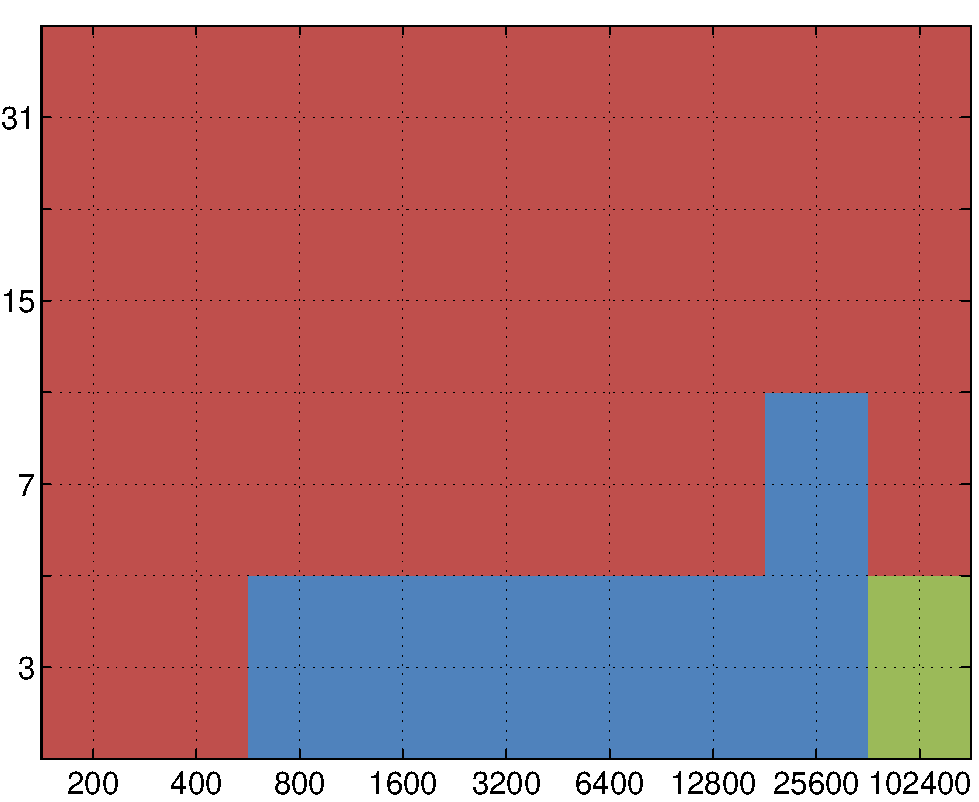
\includegraphics[width=0.5\textwidth]{iso_lena256_line.pdf}}
	  \subfloat[]{\label{fig:iso_lena256_blurkernel7}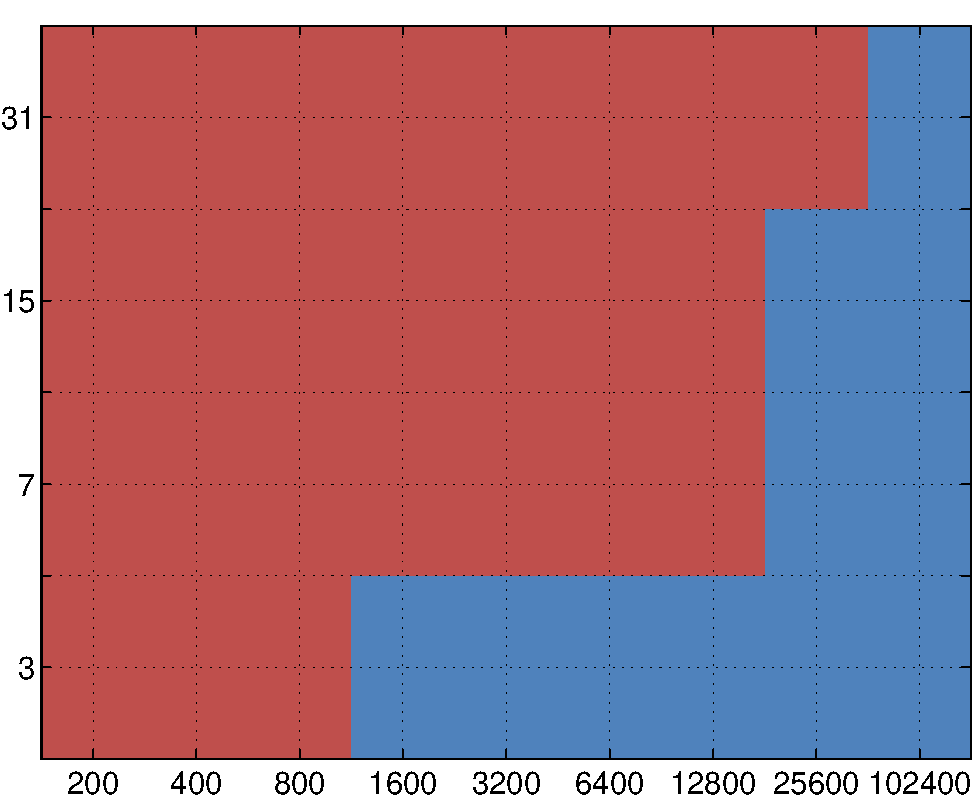
\includegraphics[width=0.5\textwidth]{iso_lena256_blurkernel7.pdf}}

	  \subfloat[]{\label{fig:iso_lena256_blurkernel8}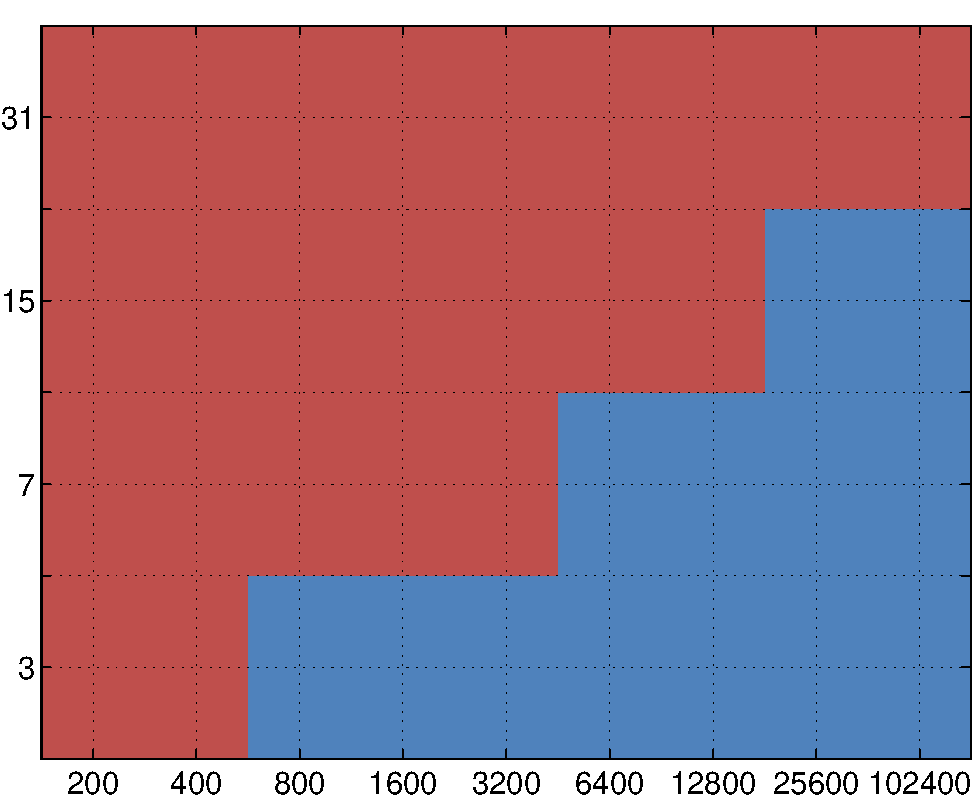
\includegraphics[width=0.5\textwidth]{iso_lena256_blurkernel8.pdf}}
	  \subfloat[]{\label{fig:iso_lena256_blurkernel10}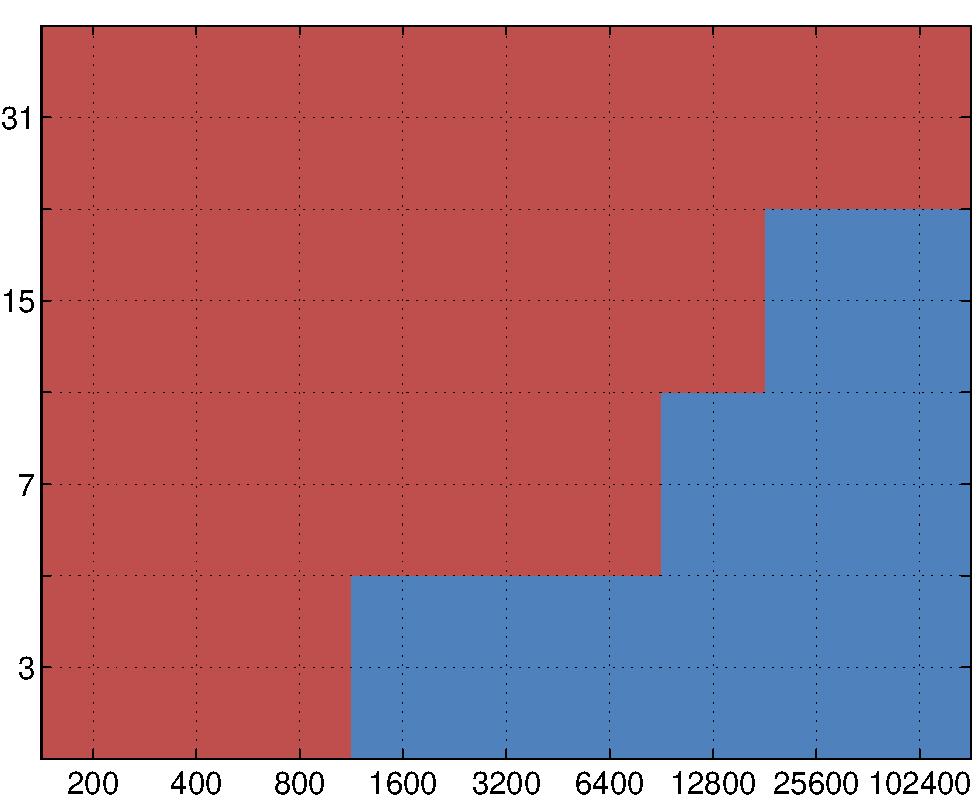
\includegraphics[width=0.5\textwidth]{iso_lena256_blurkernel10.pdf}}
  \caption[Results for the lena image in ISO mode.]{Results of the simulated data experiment on the lena image in ISO mode.}
  \end{center}
  \label{fig:iso_lena256}
\end{figure}



\begin{figure}[htb]
  \begin{center}
	  \subfloat[]{\label{fig:var_lena256_line}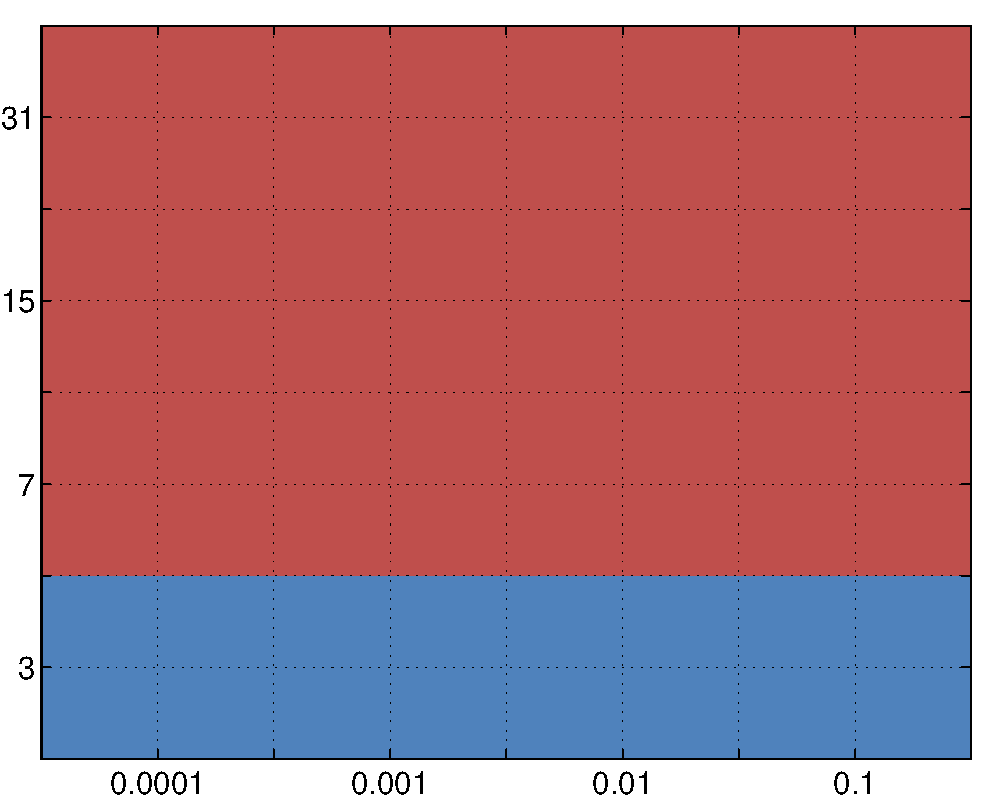
\includegraphics[width=0.5\textwidth]{var_lena256_line.pdf}}
	  \subfloat[]{\label{fig:var_lena256_blurkernel7}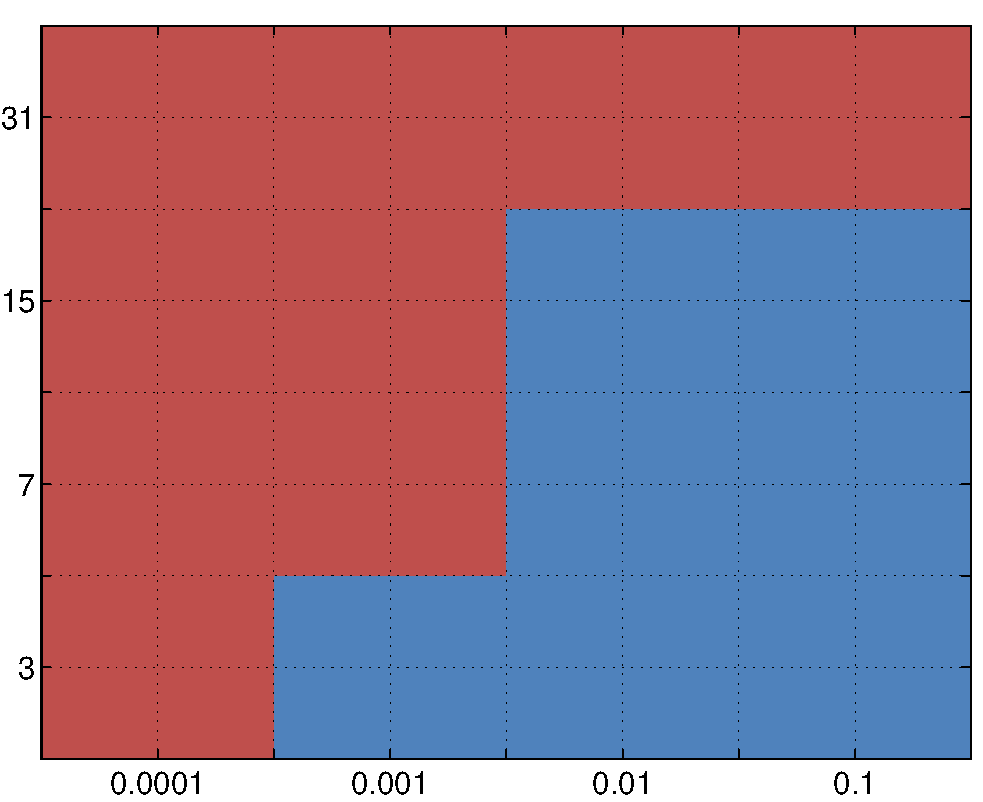
\includegraphics[width=0.5\textwidth]{var_lena256_blurkernel7.pdf}}

	  \subfloat[]{\label{fig:var_lena256_blurkernel8}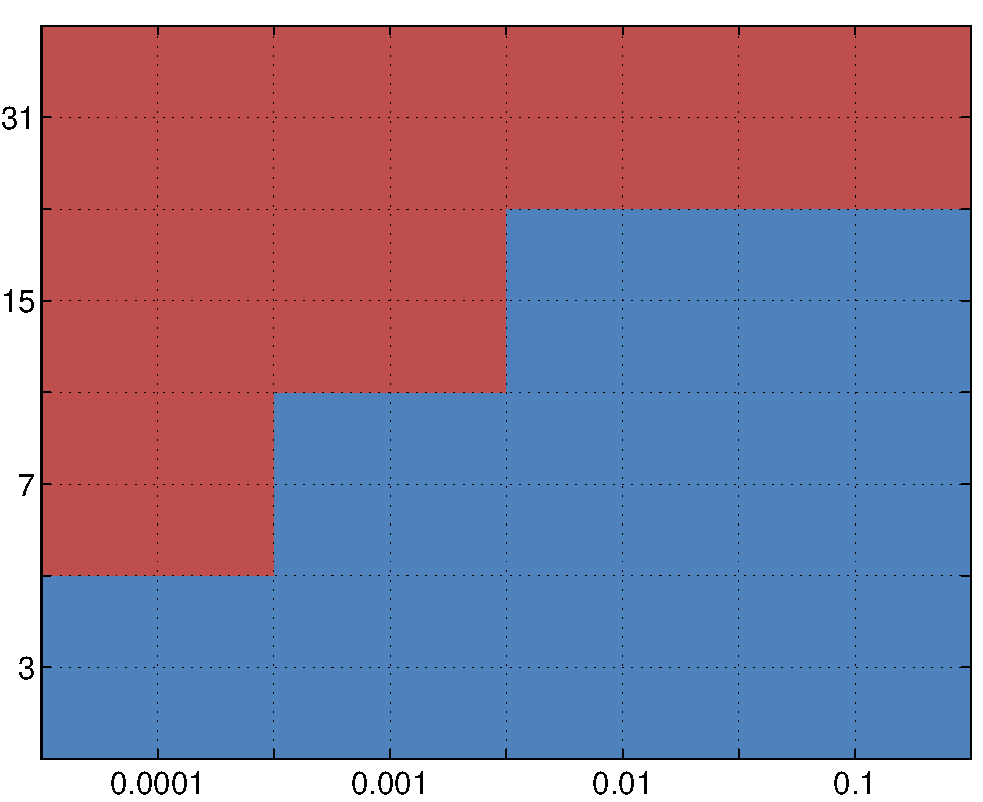
\includegraphics[width=0.5\textwidth]{var_lena256_blurkernel8.pdf}}
	  \subfloat[]{\label{fig:var_lena256_blurkernel10}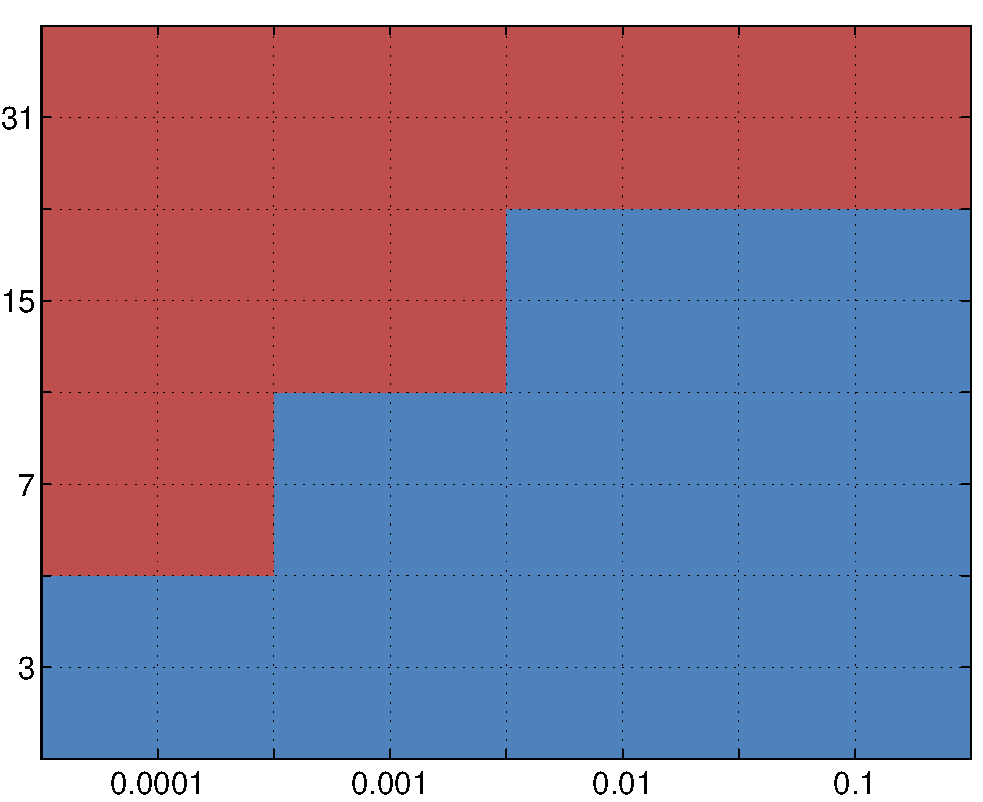
\includegraphics[width=0.5\textwidth]{var_lena256_blurkernel10.pdf}}
  \caption[Results for the lena image in variance mode.]{Results of the simulated data experiment on the lena image in variance mode.}
  \end{center}
  \label{fig:var_lena256}
\end{figure}

\clearpage

\begin{figure}[htb]
  \begin{center}
	  \subfloat[]{\label{fig:iso_castle256_line}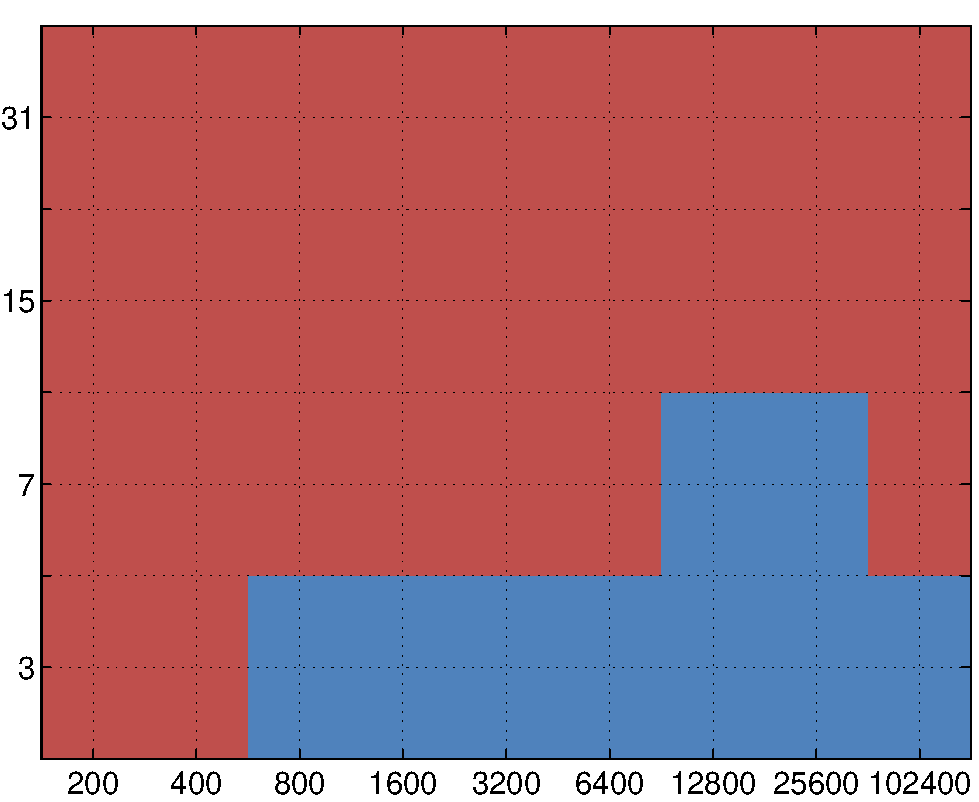
\includegraphics[width=0.5\textwidth]{iso_castle256_line.pdf}}
	  \subfloat[]{\label{fig:iso_castle256_blurkernel7}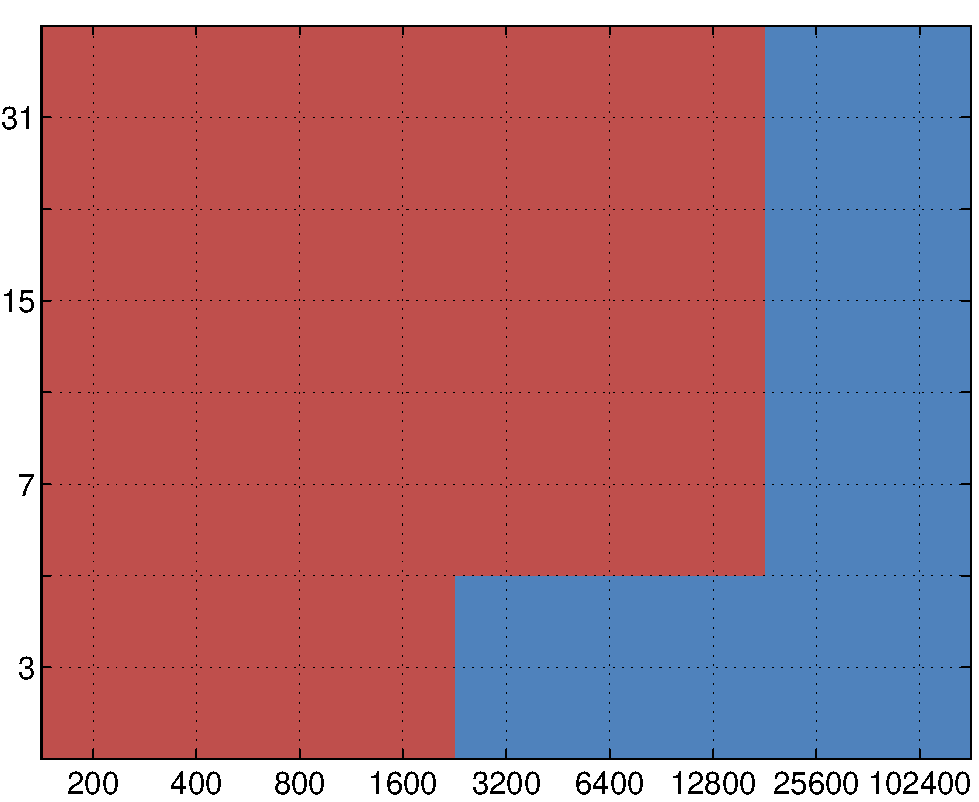
\includegraphics[width=0.5\textwidth]{iso_castle256_blurkernel7.pdf}}

	  \subfloat[]{\label{fig:iso_castle256_blurkernel8}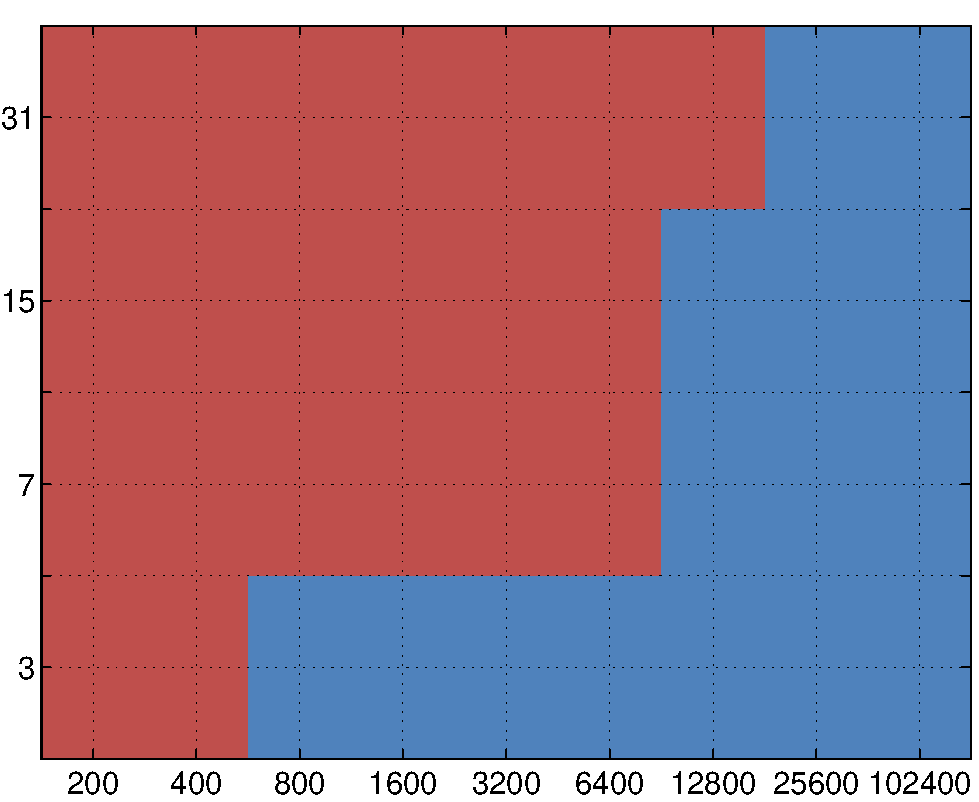
\includegraphics[width=0.5\textwidth]{iso_castle256_blurkernel8.pdf}}
	  \subfloat[]{\label{fig:iso_castle256_blurkernel10}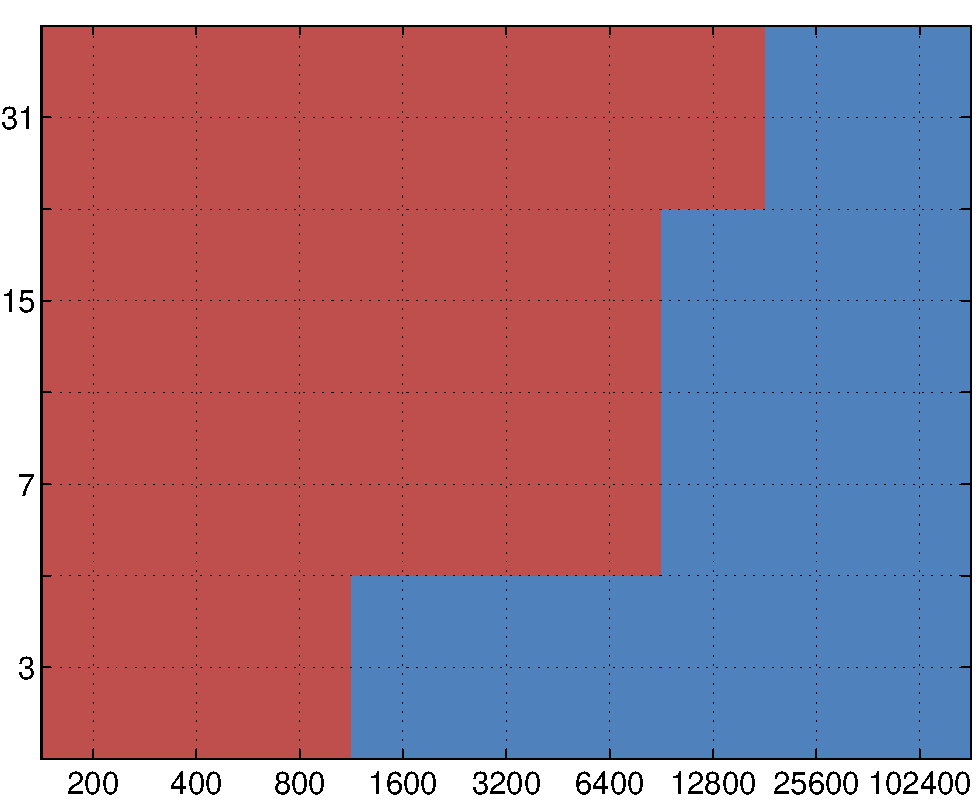
\includegraphics[width=0.5\textwidth]{iso_castle256_blurkernel10.pdf}}
  \caption[Results for the castle image in ISO mode.]{Results of the simulated data experiment on the castle image in ISO mode.}
  \end{center}
  \label{fig:iso_castle256}
\end{figure}



\begin{figure}[htb]
  \begin{center}
	  \subfloat[]{\label{fig:var_castle256_line}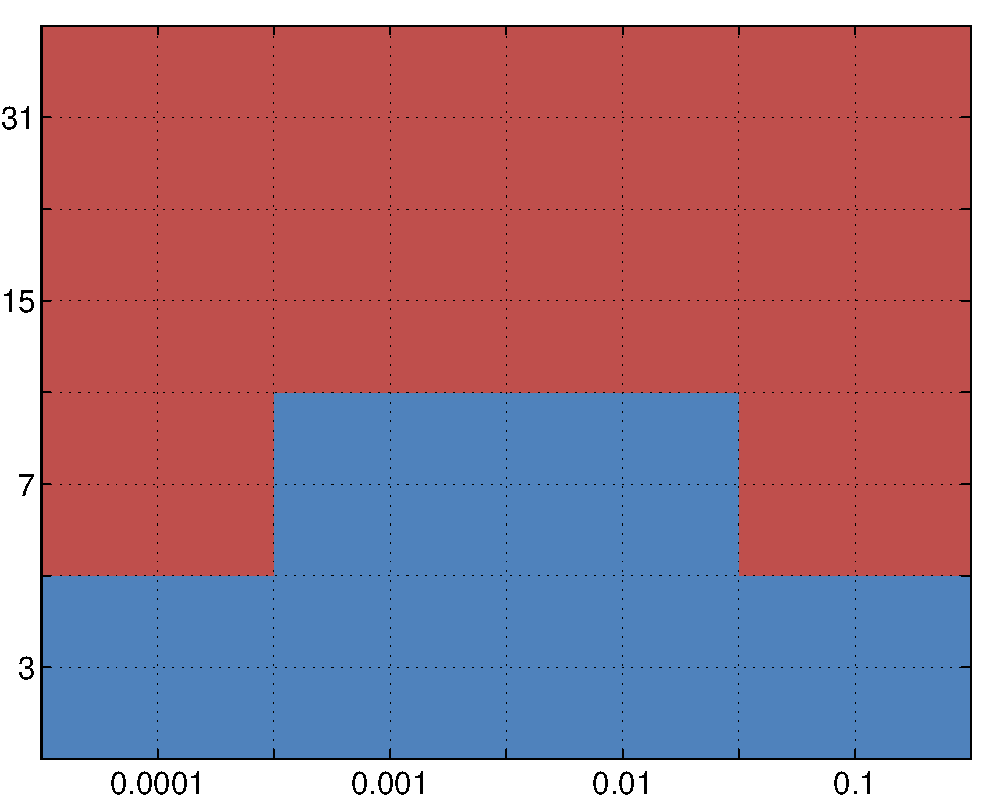
\includegraphics[width=0.5\textwidth]{var_castle256_line.pdf}}
	  \subfloat[]{\label{fig:var_castle256_blurkernel7}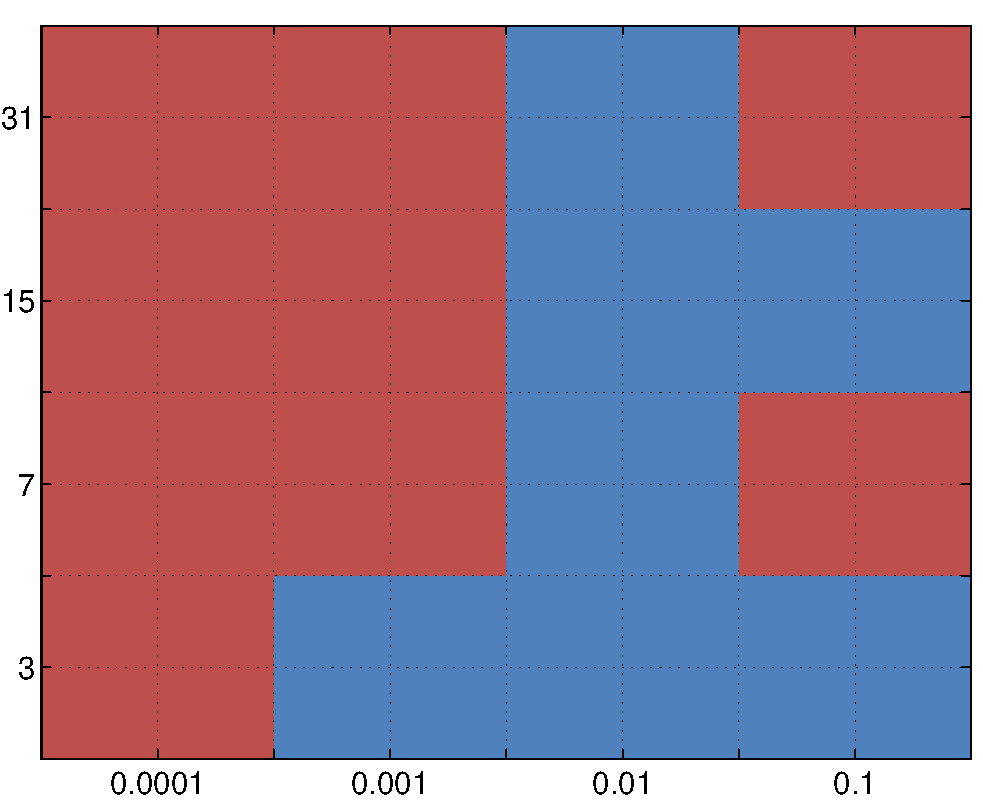
\includegraphics[width=0.5\textwidth]{var_castle256_blurkernel7.pdf}}

	  \subfloat[]{\label{fig:var_castle256_blurkernel8}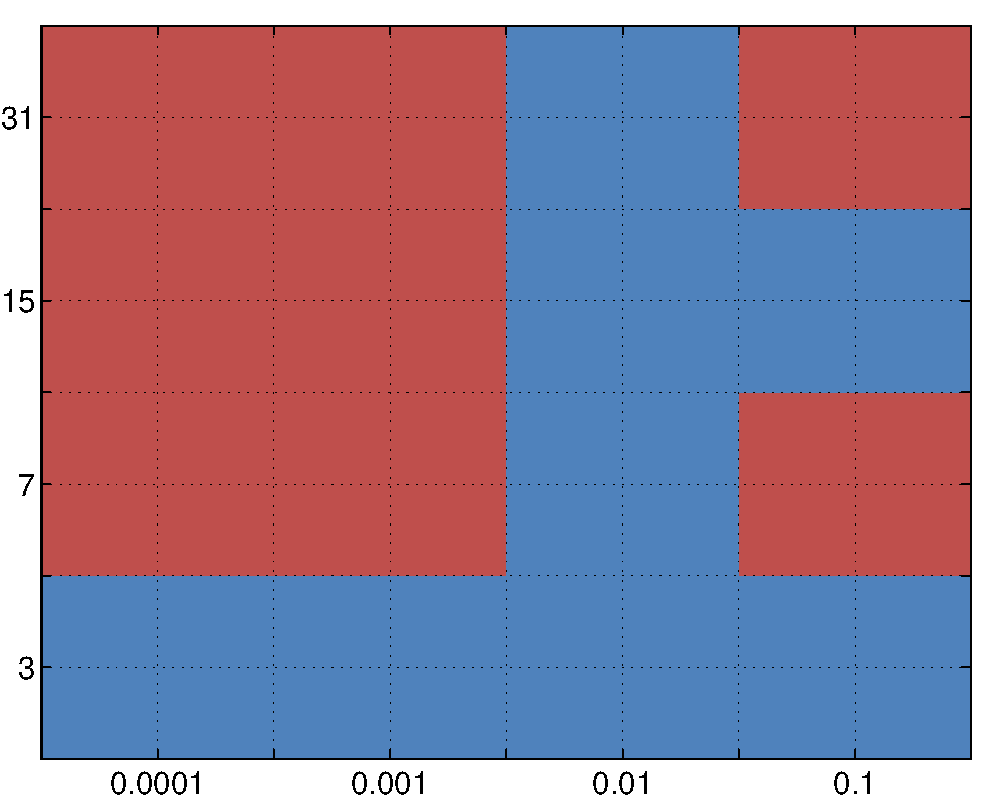
\includegraphics[width=0.5\textwidth]{var_castle256_blurkernel8.pdf}}
	  \subfloat[]{\label{fig:var_castle256_blurkernel10}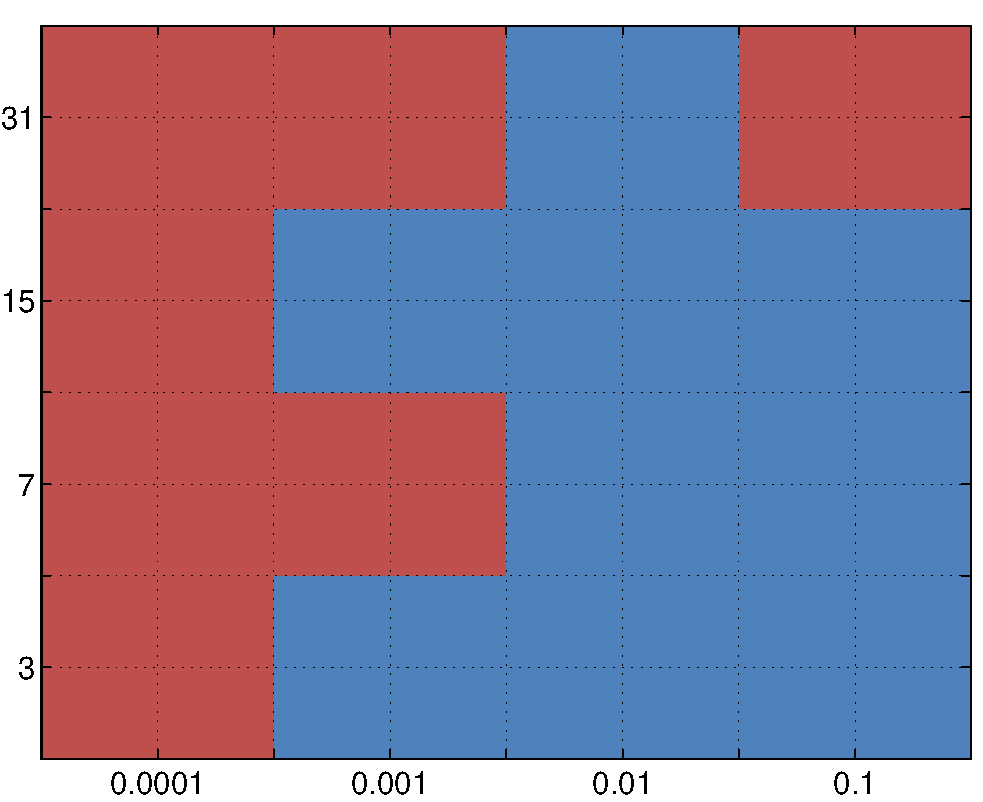
\includegraphics[width=0.5\textwidth]{var_castle256_blurkernel10.pdf}}
  \caption[Results for the castle image in variance mode.]{Results of the simulated data experiment on the castle image in variance mode.}
  \end{center}
  \label{fig:var_castle256}
\end{figure}

\clearpage

\begin{figure}[htb]
  \begin{center}
	  \subfloat[]{\label{fig:iso_text256_line}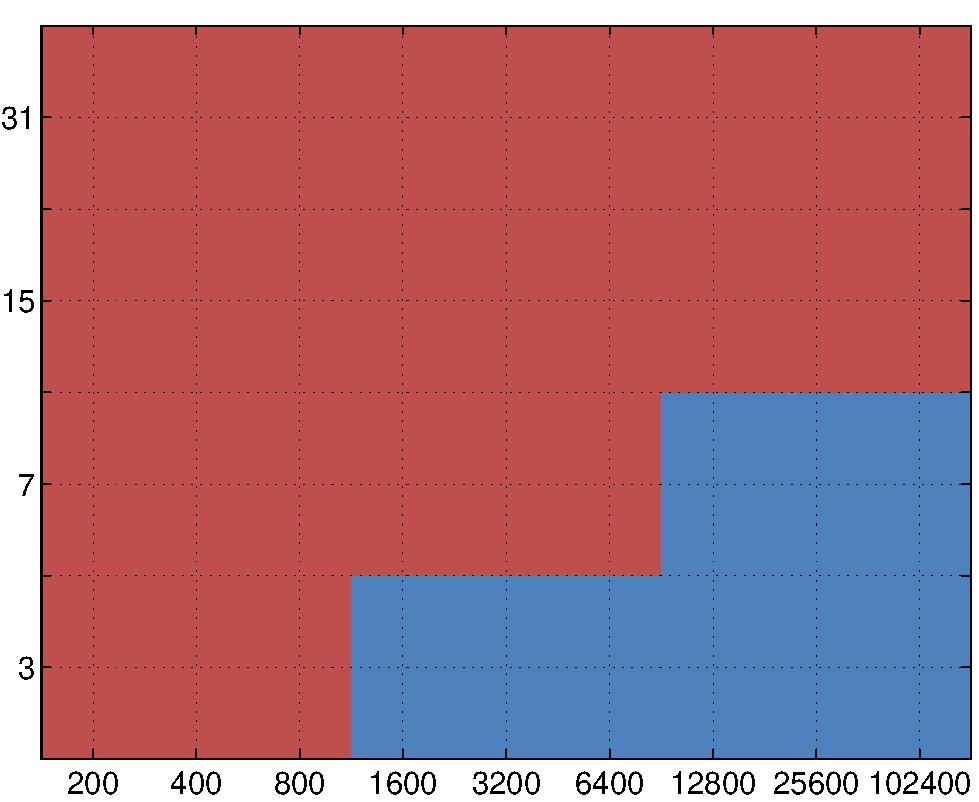
\includegraphics[width=0.5\textwidth]{iso_text256_line.pdf}}
	  \subfloat[]{\label{fig:iso_text256_blurkernel7}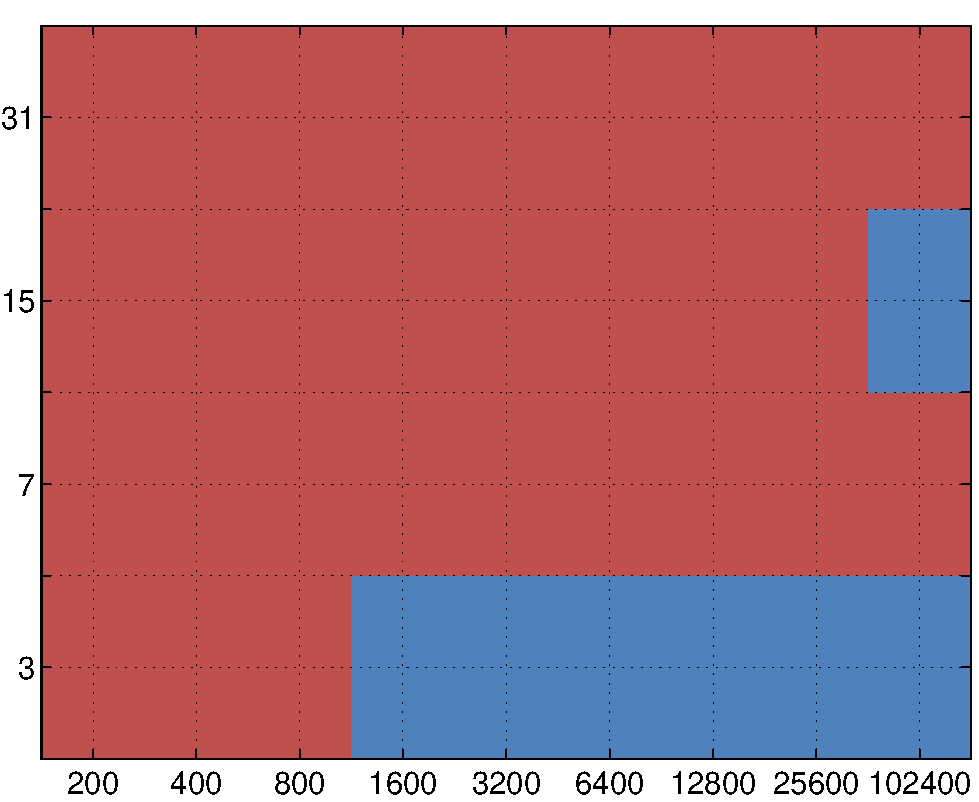
\includegraphics[width=0.5\textwidth]{iso_text256_blurkernel7.pdf}}

	  \subfloat[]{\label{fig:iso_text256_blurkernel8}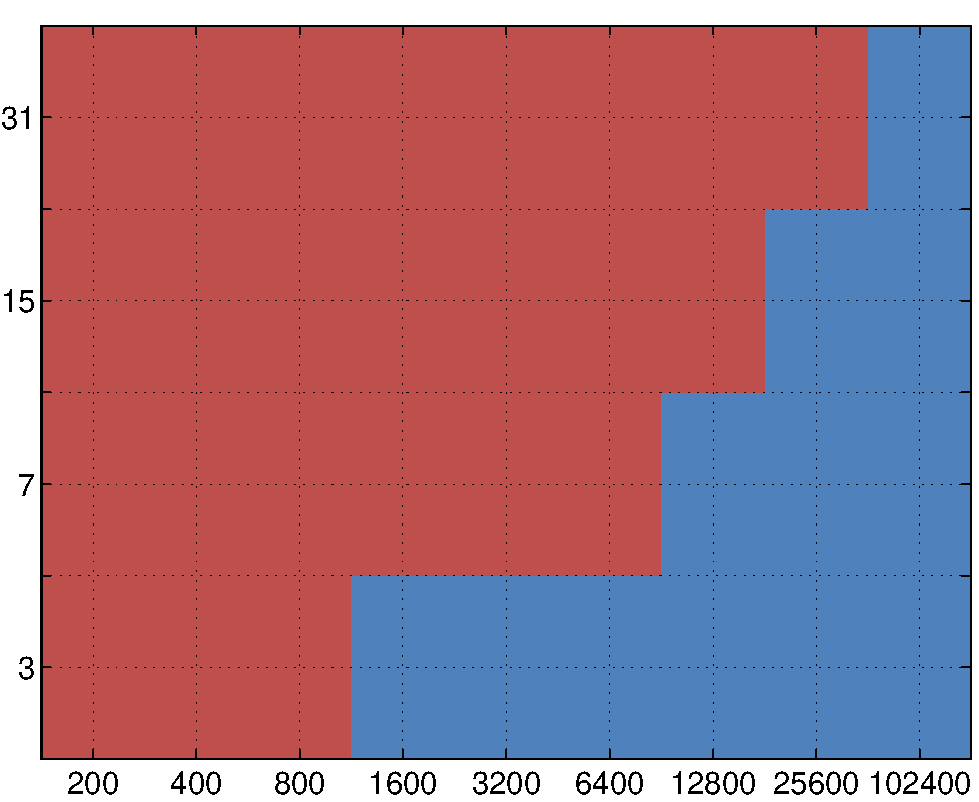
\includegraphics[width=0.5\textwidth]{iso_text256_blurkernel8.pdf}}
	  \subfloat[]{\label{fig:iso_text256_blurkernel10}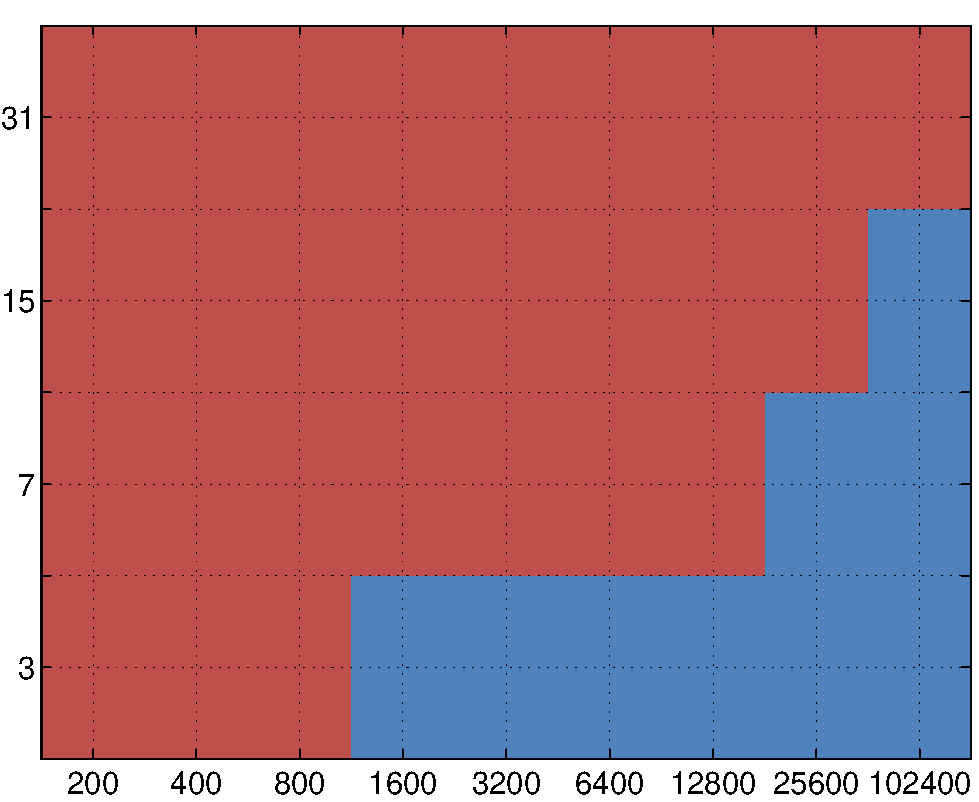
\includegraphics[width=0.5\textwidth]{iso_text256_blurkernel10.pdf}}
  \caption[Results for the text image in ISO mode.]{Results of the simulated data experiment on the text image in ISO mode.}
  \end{center}
  \label{fig:iso_text256}
\end{figure}



\begin{figure}[htb]
  \begin{center}
	  \subfloat[]{\label{fig:var_text256_line}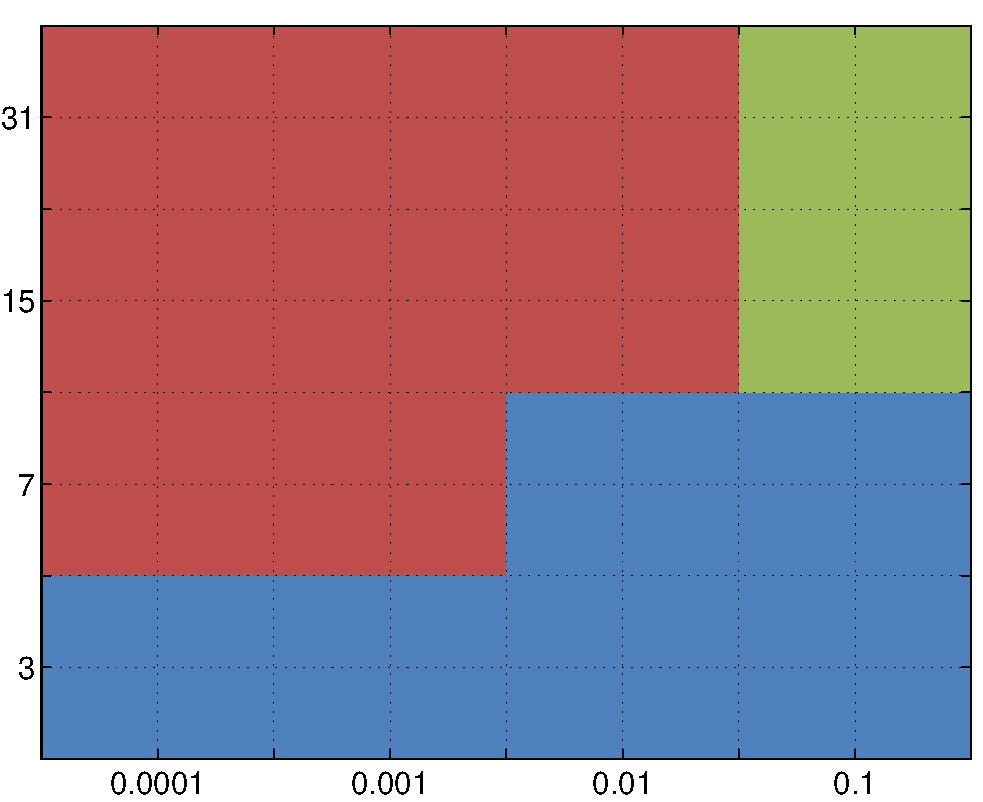
\includegraphics[width=0.5\textwidth]{var_text256_line.pdf}}
	  \subfloat[]{\label{fig:var_text256_blurkernel7}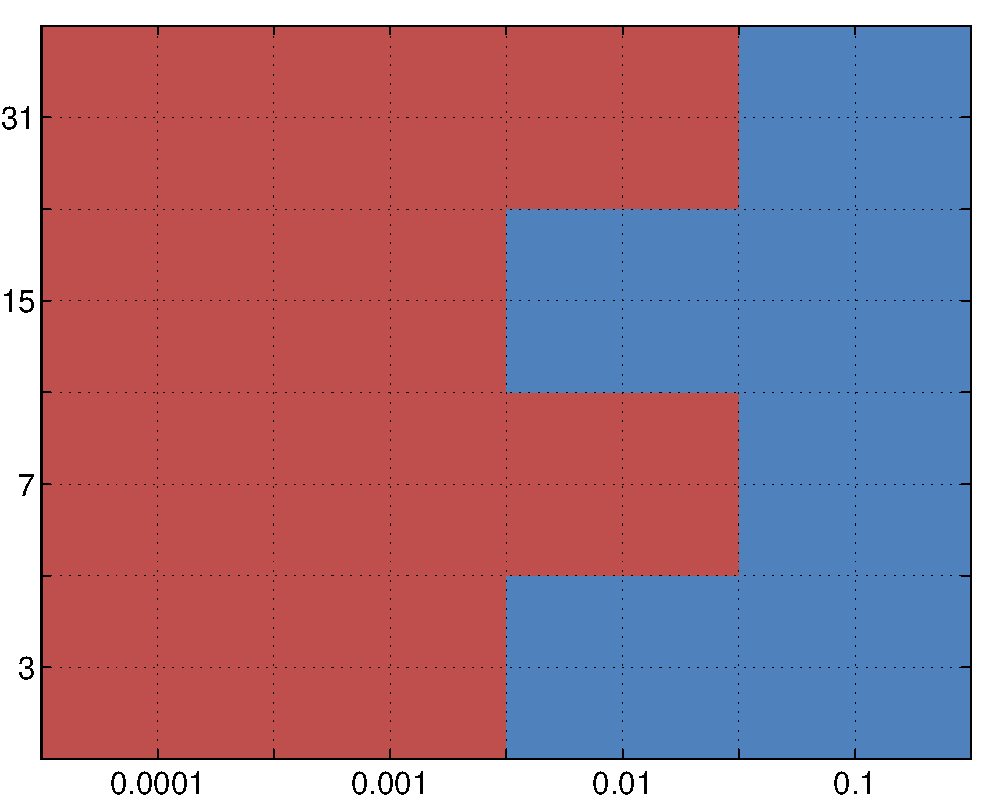
\includegraphics[width=0.5\textwidth]{var_text256_blurkernel7.pdf}}

	  \subfloat[]{\label{fig:var_text256_blurkernel8}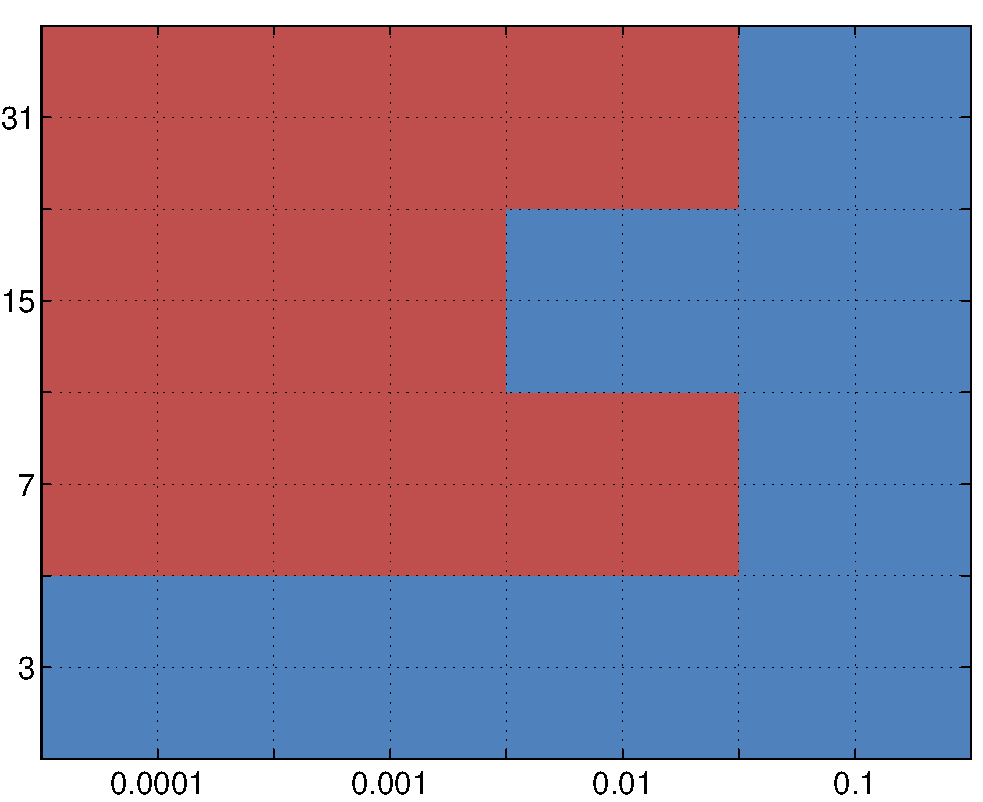
\includegraphics[width=0.5\textwidth]{var_text256_blurkernel8.pdf}}
	  \subfloat[]{\label{fig:var_text256_blurkernel10}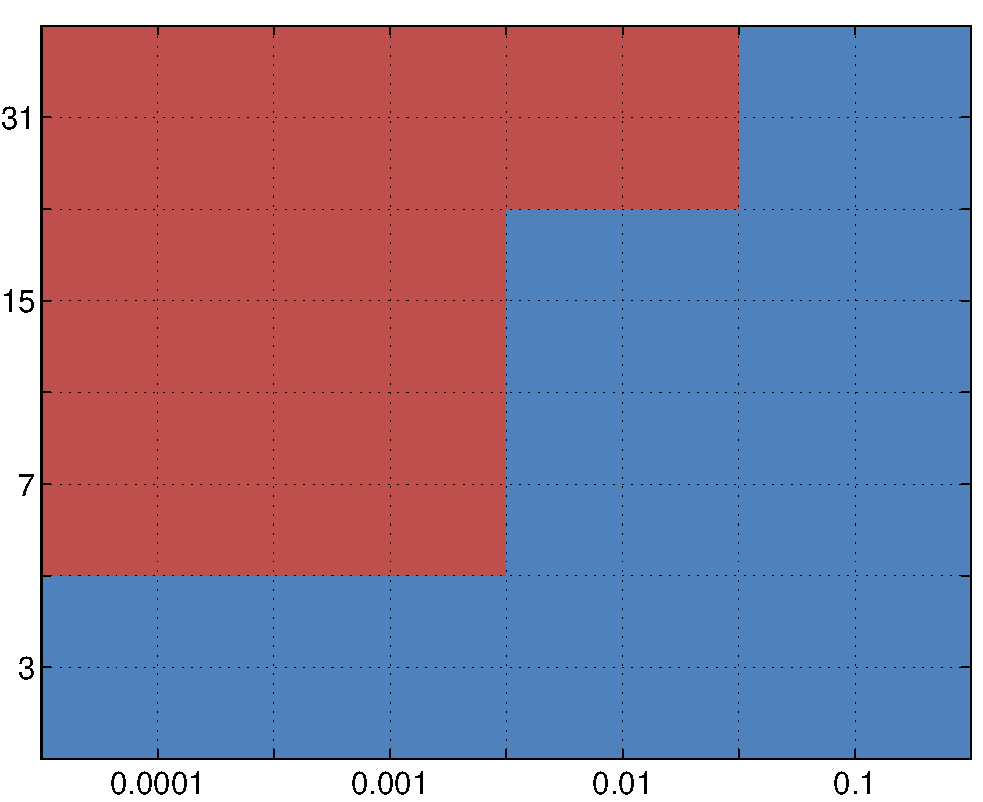
\includegraphics[width=0.5\textwidth]{var_text256_blurkernel10.pdf}}
  \caption[Results for the text image in variance mode.]{Results of the simulated data experiment on the text image in variance mode.}
  \end{center}
  \label{fig:var_text256}
\end{figure}


\clearpage

\begin{figure}[htb]
  \begin{center}
	  \subfloat[]{\label{fig:iso_tree256_line}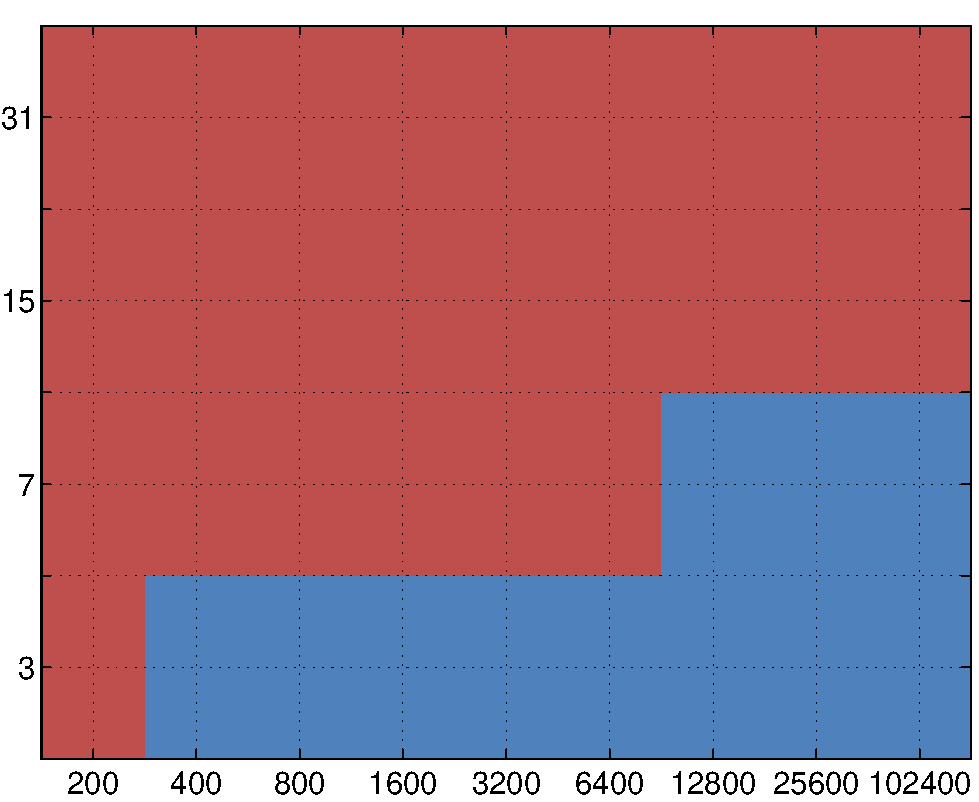
\includegraphics[width=0.5\textwidth]{iso_tree256_line.pdf}}
	  \subfloat[]{\label{fig:iso_tree256_blurkernel7}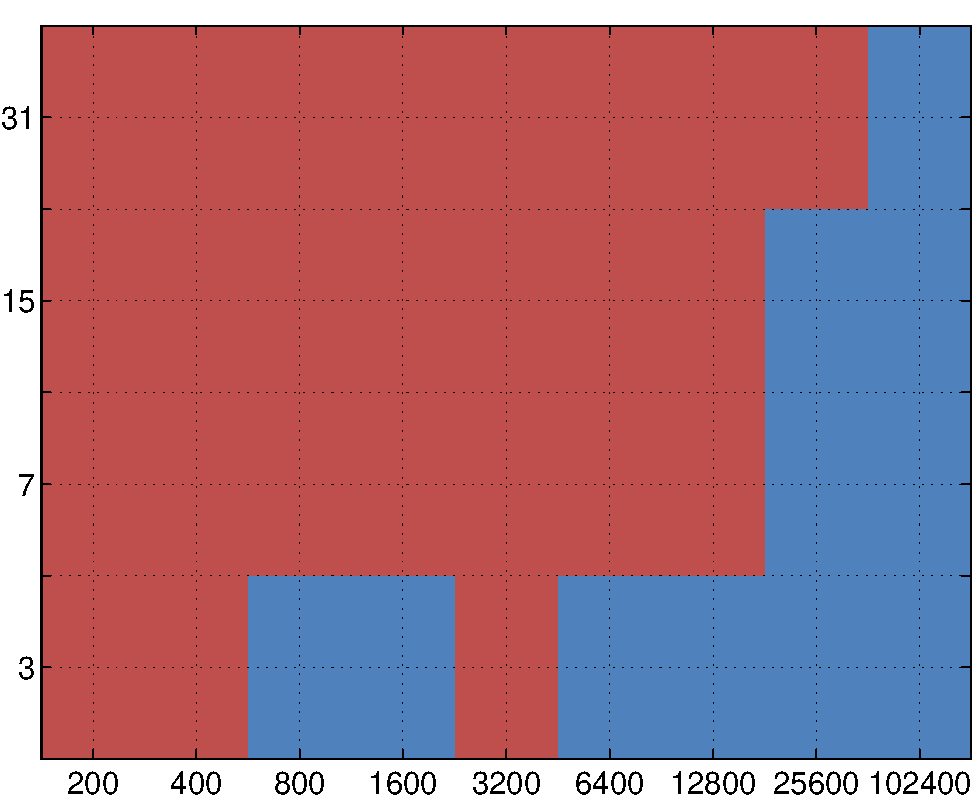
\includegraphics[width=0.5\textwidth]{iso_tree256_blurkernel7.pdf}}

	  \subfloat[]{\label{fig:iso_tree256_blurkernel8}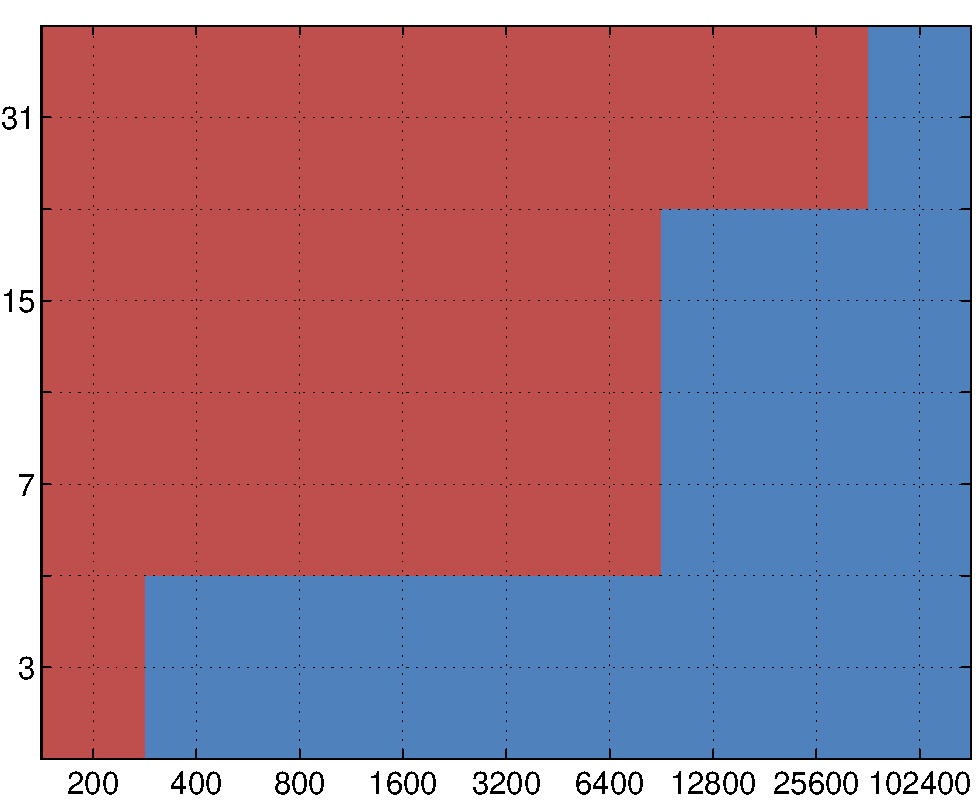
\includegraphics[width=0.5\textwidth]{iso_tree256_blurkernel8.pdf}}
	  \subfloat[]{\label{fig:iso_tree256_blurkernel10}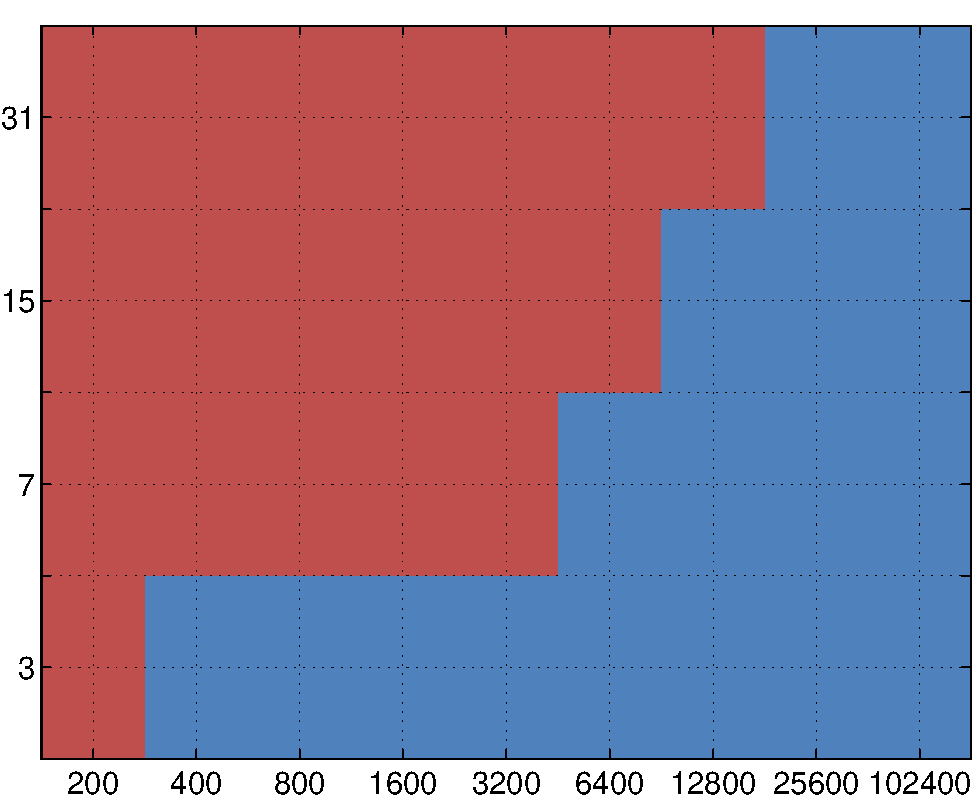
\includegraphics[width=0.5\textwidth]{iso_tree256_blurkernel10.pdf}}
  \caption[Results for the tree image in ISO mode.]{Results of the simulated data experiment on the tree image in ISO mode.}
  \end{center}
  \label{fig:iso_tree256}
\end{figure}



\begin{figure}[htb]
  \begin{center}
	  \subfloat[]{\label{fig:var_tree256_line}\includegraphics[width=0.5\textwidth]{var_tree256_line.pdf}}
	  \subfloat[]{\label{fig:var_tree256_blurkernel7}\includegraphics[width=0.5\textwidth]{var_tree256_blurkernel7.pdf}}

	  \subfloat[]{\label{fig:var_tree256_blurkernel8}\includegraphics[width=0.5\textwidth]{var_tree256_blurkernel8.pdf}}
	  \subfloat[]{\label{fig:var_tree256_blurkernel10}\includegraphics[width=0.5\textwidth]{var_tree256_blurkernel10.pdf}}
  \caption[Results for the tree image in variance mode.]{Results of the simulated data experiment on the tree image in variance mode.}
  \end{center}
  \label{fig:var_tree256}
\end{figure}

\clearpage

\section{Results for real-world data}
\label{sec:real_world_data}

As we've mentioned earlier, we'd performed 3 experiments, one for each input image multiplier value.   

\noindent \textbf{Experiment 1}, multiplier 0.125.

In this experiment, we simulated extremely low-light conditions, which is evident from the 2.5 second exposure time needed to obtain the blurred image with ISO set to 100. The noisy image was obtained with the ISO setting of 1600 and $1/6$ second exposure time. The blurred image's blur kernel size was determined to be 31 by 31 pixels, blurring was also present in the noisy image with blur kernel size 9 by 9 pixels. Setting the ISO to a higher value would have eventually removed blurring in the noisy image completely, we were however limited by the highest possible ISO setting of the camera, which was 1600. The original unmodified blurred and noisy image pair, albeit converted to grayscale, is illustrated in figure \ref{fig:experiment_001_blurred_noisy}. The experiment's result images are shown in figure \ref{fig:experiment_001_complete}. Experiment statistics are listed in table \ref{tab:experiment_001_statistics}. 

%%%
\begin{figure}[htb]
 \begin{center}
  \includegraphics[width=12cm]{experiment_001_blurred_noisy.png}
 \end{center}
 \caption{The original blurred-noisy image pair from experiment 1.}
 \label{fig:experiment_001_blurred_noisy}
\end{figure}
%%%

%%
% \begin{figure}[htb]
 % \begin{center}
  % \includegraphics[width=12cm]{experiment_001_complete.png}
 % \end{center}
 % \caption{Experiment 1.}
 % \label{fig:experiment_001_complete}
% \end{figure}
%%

%% subfloat version
\begin{figure}[htb]
  \begin{center}
	  \subfloat[]{\label{fig:experiment_001_blurred}\includegraphics[width=0.3\textwidth]{experiment_001_blurred.png}}
	  ~
	  \subfloat[]{\label{fig:experiment_001_psfs}\includegraphics[width=0.3\textwidth]{experiment_001_psfs.png}}
	  ~
	  \subfloat[]{\label{fig:experiment_001_noisy}\includegraphics[width=0.3\textwidth]{experiment_001_noisy.png}}

	  \subfloat[]{\label{fig:experiment_001_tico09}\includegraphics[width=0.3\textwidth]{experiment_001_tico09.png}}
	  ~
	  \subfloat[]{\label{fig:experiment_001_srou03}\includegraphics[width=0.3\textwidth]{experiment_001_srou03.png}}
	  ~
	  \subfloat[]{\label{fig:experiment_001_bm3d}\includegraphics[width=0.3\textwidth]{experiment_001_bm3d.png}}
  \caption[Experiment 1.]{Experiment 1.}
  \end{center}
  \label{fig:experiment_001_complete}
\end{figure}


%%%
\begin{table}[htb]
  \begin{center}
  \begin{tabular}{ | l | c | c | c | c | c | c | }
    \hline
		& Original & Blurred & Noisy & Šroubek & Tico & BM3D \\ \hline 
	Mean & 0.4884 & 0.5751 & 0.5256 &  & 0.5256 & 0.5256 \\ \hline 
	Std & 0.1859 & 0.1466 & 0.1903 &  & 0.1890 & 0.1899 \\ \hline 
	IMM96 std & 0.0093 & 0.0032 & 0.0090 &  & 0.0041 & 0.0019 \\ \hline 
	TAI98 std  & 0.0062 & 0.0029 & 0.0079 &  & 0.0035 & 0.0013 \\ \hline 
	DWT07 std  & 0.0087 & 0.0058 & 0.0145 &  & 0.0083 & 0.0062 \\ \hline 
	SWT07 std & 0.0087 & 0.0058 & 0.0145 &  & 0.0085 & 0.0063 \\ \hline 
	Avg est std & 0.0082 & 0.0044 & 0.0115 &  & 0.0061 & 0.0039 \\ \hline 
	Exp std & - &  &  & - & - & - \\ \hline 
	SNR     & - & 3.4323 & 11.0442 &  & 10.9282 & 11.1391 \\ \hline 
	Gamma & - & - & - &  & - & - \\ \hline 
	Lambda & - & - & - &  & - & - \\ \hline 

  \end{tabular}
  \end{center}
  \caption{Image statistics for experiment 1.}
  \label{tab:experiment_001_statistics}
\end{table}
%%%


\noindent \textbf{Experiment 2}, multiplier 0.25.

In this case, the blurred image was obtained using the ISO setting of 100 and 1 second exposure time. The noisy image was again obtained with the ISO setting of 1600 and $1/15$ second exposure time. The blurred image's blur kernel size was determined to be 21 by 21 pixels, blurring in the noisy image was also present, at 5 by 5 pixels. The original blurred and noisy image pair (converted to grayscale), is illustrated in figure \ref{fig:experiment_002_blurred_noisy}. Resulting images are shown in figure \ref{fig:experiment_002_complete} and their statistics are listed in table \ref{tab:experiment_002_statistics}.

%%%
\begin{figure}[htb]
 \begin{center}
  \includegraphics[width=12cm]{experiment_002_blurred_noisy.png}
 \end{center}
 \caption{The original blurred-noisy image pair from experiment 2.}
 \label{fig:experiment_002_blurred_noisy}
\end{figure}
%%%

%%
% \begin{figure}[htb]
 % \begin{center}
  % \includegraphics[width=12cm]{experiment_002_complete.png}
 % \end{center}
 % \caption{Experiment 2.}
 % \label{fig:experiment_002_complete}
% \end{figure}
%%

%% subfloat version
\begin{figure}[htb]
  \begin{center}
	  \subfloat[]{\label{fig:experiment_002_blurred}\includegraphics[width=0.3\textwidth]{experiment_002_blurred.png}}
	  ~
	  \subfloat[]{\label{fig:experiment_002_psfs}\includegraphics[width=0.3\textwidth]{experiment_002_psfs.png}}
	  ~
	  \subfloat[]{\label{fig:experiment_002_noisy}\includegraphics[width=0.3\textwidth]{experiment_002_noisy.png}}

	  \subfloat[]{\label{fig:experiment_002_tico09}\includegraphics[width=0.3\textwidth]{experiment_002_tico09.png}}
	  ~
	  \subfloat[]{\label{fig:experiment_002_srou03}\includegraphics[width=0.3\textwidth]{experiment_002_srou03.png}}
	  ~
	  \subfloat[]{\label{fig:experiment_002_bm3d}\includegraphics[width=0.3\textwidth]{experiment_002_bm3d.png}}
  \caption[Experiment 2.]{Experiment 2.}
  \end{center}
  \label{fig:experiment_002_complete}
\end{figure}



%%%
\begin{table}[htb]
  \begin{center}
  \begin{tabular}{ | l | c | c | c | c | c | c | }
    \hline
		& Original & Blurred & Noisy & Šroubek & Tico & BM3D \\ \hline 
	Mean & 0.4884 & 0.6560 & 0.6488 &  & 0.6488 & 0.6488 \\ \hline 
	Std & 0.1859 & 0.1977 & 0.2422 &  & 0.2401 & 0.2419 \\ \hline 
	IMM96 std & 0.0093 & 0.0031 & 0.0095 &  & 0.0052 & 0.0042 \\ \hline 
	TAI98 std  & 0.0062 & 0.0026 & 0.0077 &  & 0.0041 & 0.0027 \\ \hline 
	DWT07 std  & 0.0087 & 0.0058 & 0.0116 &  & 0.0079 & 0.0067 \\ \hline 
	SWT07 std & 0.0087 & 0.0058 & 0.0116 &  & 0.0081 & 0.0067 \\ \hline 
	Avg est std & 0.0082 & 0.0043 & 0.0101 &  & 0.0063 & 0.0051 \\ \hline 
	Exp std & - &  &  & - & - & - \\ \hline 
	SNR     & - & 4.8812 & 10.5967 &  & 10.5525 & 10.6172 \\ \hline 
	Gamma & - & - & - &  & - & - \\ \hline 
	Lambda & - & - & - &  & - & - \\ \hline 

  \end{tabular}
  \end{center}
  \caption{Image statistics for experiment 2.}
  \label{tab:experiment_002_statistics}
\end{table}
%%%

\noindent \textbf{Experiment 3}, multiplier 0.5.

The blurred image was taken using the ISO setting of 100 and $1/3$ second exposure time, resulting in a blur kernel 17 by 17 pixels in size. The noisy image, obtained with the ISO setting of 1000 and $1/30$ second exposure time, was blurred by a kernel 5 by 5 pixels in size. The original grayscale blurred and noisy image pair is illustrated in figure \ref{fig:experiment_003_blurred_noisy}. Resulting images are shown in figure \ref{fig:experiment_003_complete}. Experiment statistics are listed in table \ref{tab:experiment_003_statistics}.

%%%
\begin{figure}[htb]
 \begin{center}
  \includegraphics[width=12cm]{experiment_003_blurred_noisy.png}
 \end{center}
 \caption{The original blurred-noisy image pair from experiment 3.}
 \label{fig:experiment_003_blurred_noisy}
\end{figure}
%%%

%%
% \begin{figure}[htb]
 % \begin{center}
  % \includegraphics[width=12cm]{experiment_003_complete.png}
 % \end{center}
 % \caption{Experiment 3.}
 % \label{fig:experiment_003_complete}
% \end{figure}
%%

%% subfloat version
\begin{figure}[htb]
  \begin{center}
	  \subfloat[]{\label{fig:experiment_003_blurred}\includegraphics[width=0.3\textwidth]{experiment_003_blurred.png}}
	  ~
	  \subfloat[]{\label{fig:experiment_003_psfs}\includegraphics[width=0.3\textwidth]{experiment_003_psfs.png}}
	  ~
	  \subfloat[]{\label{fig:experiment_003_noisy}\includegraphics[width=0.3\textwidth]{experiment_003_noisy.png}}

	  \subfloat[]{\label{fig:experiment_003_tico09}\includegraphics[width=0.3\textwidth]{experiment_003_tico09.png}}
	  ~
	  \subfloat[]{\label{fig:experiment_003_srou03}\includegraphics[width=0.3\textwidth]{experiment_003_srou03.png}}
	  ~
	  \subfloat[]{\label{fig:experiment_003_bm3d}\includegraphics[width=0.3\textwidth]{experiment_003_bm3d.png}}
  \caption[Experiment 3.]{Experiment 3.}
  \end{center}
  \label{fig:experiment_003_complete}
\end{figure}


%%%
\begin{table}[htb]
	\begin{center}
	\begin{tabular}{ | l | c | c | c | c | c | c | }
	\hline
		& Original & Blurred & Noisy & Šroubek & Tico & BM3D \\ \hline 
	Mean & 0.4884 & 0.7700 & 0.6879 &  & 0.6879 & 0.6879 \\ \hline 
	Std & 0.1859 & 0.1798 & 0.2304 &  & 0.2286 & 0.2302 \\ \hline 
	IMM96 std & 0.0093 & 0.0030 & 0.0074 &  & 0.0049 & 0.0032 \\ \hline 
	TAI98 std  & 0.0062 & 0.0025 & 0.0057 &  & 0.0037 & 0.0019 \\ \hline 
	DWT07 std  & 0.0087 & 0.0058 & 0.0116 &  & 0.0072 & 0.0056 \\ \hline 
	SWT07 std & 0.0087 & 0.0058 & 0.0116 &  & 0.0074 & 0.0057 \\ \hline 
	Avg est std & 0.0082 & 0.0043 & 0.0091 &  & 0.0058 & 0.0041 \\ \hline 
	Exp std & - &  &  & - & - & - \\ \hline 
	SNR     & - & 3.8498 & 9.1393 &  & 9.1761 & 9.1493 \\ \hline 
	Gamma & - & - & - &  & - & - \\ \hline 
	Lambda & - & - & - &  & - & - \\ \hline 

	\end{tabular}
	\end{center}
	\caption{Image statistics for experiment 3.}
	\label{tab:experiment_003_statistics}
\end{table}
%%%

\section{Evaluation}
\label{sec:evaluation}

From simulated experimental data, we observe that on average, the presence of noise has a greater influence on the eventual outcome of a particular method than the extent of blurring does. This is evident from figures \ref{fig:avg_methods_vs_var}, \ref{fig:avg_methods_vs_ISO}, \ref{fig:avg_methods_vs_psf_size} and \ref{fig:avg_methods_vs_ISO_psf_size}. Results of the BM3D denoising algorithm are completely independent of the blur PSF size, since the algorithm is executed solely on the noisy, blurless image. 

%%%
\begin{figure}[htb]
 \begin{center}
  \includegraphics[width=12cm]{avg_methods_vs_var.pdf}
 \end{center}
 \caption{Average dependence of tested algorithms on the level of noise.}
 \label{fig:avg_methods_vs_var}
\end{figure}
%%%

%%%
\begin{figure}[htb]
 \begin{center}
  \includegraphics[width=12cm]{avg_methods_vs_ISO.pdf}
 \end{center}
 \caption{Average dependence of tested algorithms on the input ISO.}
 \label{fig:avg_methods_vs_ISO}
\end{figure}
%%%

%%%
\begin{figure}[htb]
 \begin{center}
  \includegraphics[width=12cm]{avg_methods_vs_var_psf_size.pdf}
 \end{center}
 \caption{Average dependence of tested algorithms on the size of blurring (for variance data).}
 \label{fig:avg_methods_vs_psf_size}
\end{figure}
%%%

%%%
\begin{figure}[htb]
 \begin{center}
  \includegraphics[width=12cm]{avg_methods_vs_ISO_psf_size.pdf}
 \end{center}
 \caption{Average dependence of tested algorithms on the size of blurring (for ISO data).}
 \label{fig:avg_methods_vs_ISO_psf_size}
\end{figure}
%%%

\clearpage




We've observed that the BM3D denoising algorithm provides consistent results irrespective of the underlying image (also of the type and size of the blur PSF, since blurred images were not denoised); the only exception to this rule are images that exhibit self-similar (fractal) behavior, such the as tree image used in our tests. These features disrupt the block matching process as more matching blocks are found all across the image than is normally the case. The performance of this algorithm is also dependent on the type of noise present and the precision of the estimation of noise standard deviation $\sigma$. The algorithm performs very well in case of zero mean-Gaussian additive noise (even for variances as high as 0.01) and also for most ISO values, where the noise roughly corresponds to Gaussian. In case of high variance, or non-Gaussian noise, block-matching artifacts become more evident, resulting in reduced performance, as can be seen figure \ref{fig:bm3d_failure}, which also illustrates the lowered performance on an image containing self-similarity. 

%% subfloat version
\begin{figure}[htb]
  \begin{center}
	  \subfloat[]{\label{fig:bm3d_failure_tree}\includegraphics[width=0.3\textwidth]{bm3d_failure_tree.png}}
	  ~
	  \subfloat[]{\label{fig:bm3d_failure_ISO_102400}\includegraphics[width=0.3\textwidth]{bm3d_failure_ISO_102400.png}}
	  ~
	  \subfloat[]{\label{fig:bm3d_failure_var_ISO_102400}\includegraphics[width=0.3\textwidth]{bm3d_failure_var_ISO_102400.png}}

	  \subfloat[]{\label{fig:bm3d_failure_tree_res}\includegraphics[width=0.3\textwidth]{bm3d_failure_tree_res.png}}
	  ~
	  \subfloat[]{\label{fig:bm3d_failure_ISO_102400_res}\includegraphics[width=0.3\textwidth]{bm3d_failure_ISO_102400_res.png}}
	  ~
	  \subfloat[]{\label{fig:bm3d_failure_var_ISO_102400_res}\includegraphics[width=0.3\textwidth]{bm3d_failure_var_ISO_102400_res.png}}
  \caption[Failures of the BM3D algorithm.]{Failures of the BM3D algorithm.}
  \end{center}
  \label{fig:bm3d_failure}
\end{figure}



The added value of deconvolution in case of Šroubek's algorithm is apparent in the setting of little to moderate blurring in the long-exposed image and high noise in the short exposed image. Here, the blurred image contributes information that the BM3D algorithm simply cannot obtain. In rare cases, Šroubek's algorithm outperforms the BM3D algorithm even for highly blurred images. However, a significant disadvantage of Šroubek's algorithm is the need to fine-tune the $\lambda$ and $\gamma$ parameters, since the theoretically computed ones do not produce satisfying results, as we've observed in real-world data.



Although the output of Tico's algorithm is plagued by artifacts at high noise values the algorithm itself has outperformed either Tico's or      



\chapter{Conclusion}

We have studied and described several methods of image deblurring using two images with different exposure times. We have established two categories, the {\em deconvolution} and {\em non-deconvolution} methods.  We have selected one method from each category, tested them on generated as well as real-world data and compared them to each other and to the results of a state-of-the-art denoising algorithm (BM3D) performed on the noisy image ($g_1$ from equation \ref{eq:general_model}, specifically). We have, given the experimental results, demonstrated that: 

\begin{itemize}
\item In a majority of cases, using two images with different exposure times provides no additional benefit over single-image denoising
\item Two-image deblurring algorithms “defeat” single image denoising in rare cases and in conditions too extreme to be attained by conventional photography
\item In low-noise conditions, using a {\em non-deconvolution} method generally provides better results than using a {\em deconvolution} method
\item All tested methods generally fail on data exhibiting self-similarity and other non-standard behavior rarely present in conventional photographs
\end{itemize}

This leads us to a general conclusion that an efficient single image denoising algorithm provides better results than using two images with different exposure times. 

\section{Possible future improvements}

\textbf{TODO}

\appendix

\chapter{Contents of the CD}


\chapter{Implementation and testing notes}
\label{chap:notes}

Methods tested in this thesis have been implemented using Matlab version 7.4.0 running on Microsoft Windows XP Professional SP 2. Apart from standard Matlab functions, the {\em Wavelet Toobox} and {\em Image Processing Toolbox} were used.

Tests were performed on two computers, the first being a single-core 1.8 GHz PC running 32-bit Microsoft Windows XP Professional SP 2 with 1792 MB of RAM and the second was a quad-core hyperthreaded laptop PC running 64bit 
Windows XP 7 Professional with 8192 MB of RAM, on which up to 4 virtual Windows XP Professional PCs configured to have a single processor and 1024 MB of RAM were run in parallel. Virtual Windows XP PCs were required due to the available Matlab version, which is older and incompatible with Windows 7.

The total time needed to generate all BM3D data was approximately 45 minutes, which was due to the fact that the BM3D denoising algorithm was written in C++ and provided in binary form with a MATLAB interface. In case of Tico's wavelet fusion, processing of one blurred - noisy image pair was independent of the blur size and took about 2 minutes, bringing the total time close to 28 hours. The running time of Šroubek's MC-AM algorithm was highly dependent on PSF size and doubling the PSF size approximately quadrupled the running time, which was approximately 20 - 40 (sometimes even an hour) for PSF 31 pixels in size, 5 - 10 minutes for 15, about 2 minutes for 7 and less than a minute for 3, bringing the total time to about 5 and a half days, which was effectively halved due to computations being performed on 2 PCs in parallel. Searching for the best $\lambda$ and $\gamma$ parameters for the computation of Šroubek's algorithm in case of real-world data required its complete execution for each pair; since there were approximately 200 $\lambda$ and $\gamma$ pairs tested for each experiment, the total running time was approximately 500 hours, effectively about one quarter of time was needed due to parallelization.  

No GUI was implemented and tests were performed in batch mode, results being written to a *.csv file. This is readable in plain text, but is better wieved in a spreadsheet processor, such as Microsoft Excel or Libre Office. Graphs were created in both MATLAB and Microsoft Excel 2007, both of which allow them to be created in the eps format, convertible to pdf. 

Image registration was performed directly in MATLAB using control point selection routine \texttt{cpselect} which produces a set of corresponding control points, the \texttt{cp2tform} routine, which takes the set of control points and computes an image transformation structure from them depending on the desired transformation type and the routine \texttt{imtransform}, which performs the transformation itself. Projective transformation was used as the desired transformation to correct for possible perspective deformation that could occur when projecting the image or taking picture of it.  

The thesis was developed and maintained using the Git versioning system and placed (with the exception of generated image data) into a public Git repository at \texttt{https://github.com:jozefsabo/Thesis.git} to facilitate accessibility from multiple locations.

Image editing tasks were handled in Paint.NET and IrfanView.

%%%
%%% Literatura se řadí abecedně. Úvádí se pouze literatura, na kterou se v textu odkazuje.
%%% Při odkazu na knihu se vždy uvádějí čísla stránek.

\begin{thebibliography}{xxxxx-99}
\addcontentsline{toc}{chapter}{Bibliography}
 \bibitem{jia04}Jia J., Sun J., Tang C.K., Shum H.Y.: {\em Bayesian correction of image intensity with spatial consideration}, Proceedings of the eighth European Conference on Computer Vision, 256-266, Praha, 2004
 \bibitem{rich72}Richardson, W. H.: {\em Bayesian-Based Iterative Method of Image Restoration}, JOSA, Volume 62, 2007
 \bibitem{foi07}Foi A., Trimeche M., Katkovnik V., Egiazarian K.: {\em Practical Poissonian-Gaussian noise modeling and fitting for single-image raw-data}, IEEE Transactions, 2007
 \bibitem{tico06}Tico M., Vehvilainen M.: {\em  Estimation of motion blur point spread function from differently exposed images}, Nokia Research Center, Tampere, Finland, 2006
 \bibitem{razl07}Razligh Q.R., Kehtarnavaz N.: {\em Image blur reduction for cell-phone cameras via adaptive tonal correction}, Department of Electrical Engineering, University of Texas at Dallas, 2007
 \bibitem{tico09}Tico M., Pulli K.: {\em Image enhancement via blur and noisy image fusion}, Nokia Research Center, Palo Alto, CA, USA, 2009
 \bibitem{mall09}Mallat, S.: {\em A wavelet tour of signal processing, the sparse way}, Elsevier, Burlington, MA, 2009
 \bibitem{rao90}Rao, A.R.: {\em A Taxonomy for Texture Description and Identification}, Springer Verlag, 1990
 \bibitem{liu01}Liu X., Gamal A.: {\em Simultaneous image formation and motion blur restoration via multiple capture}, Proceedings of the International Conference on Acoustics, Speech, Signal Processing, 2001
 \bibitem{yuan07}Yuan L., Sun J., Quan L., Shum H.Y.: {\em Image Deblurring with blurred/noisy image pairs},  Computer Science Department, Hong Kong University of Science and Technology, 2007
 \bibitem{tico07}Tico M., Vehvilainen M.: {\em Image stabilization based on fusing the visual information in differently exposed images}, Nokia Research Center, Tampere, Finland, 2007
 \bibitem{bene04}Beneš B., Felkel P., Sochor J., Žára J.: {\em Moderní počítačová grafika, 2. vydání}, Computer Press, 2004
 \bibitem{bied04}Biedl T., Chan T., Demaine E., Fleischer R., Golin M., King J., IanMun J.: {\em Fun Sort - or the Chaos of Unordered Binary Search},  Discrete Applied Mathematics, vol. 144, p. 231-236, 2004
 \bibitem{rein01}Gooch M., Reinhard E., Ashikmin E., Shirley P.: {\em Color transfer between images}, IEEE Computer Graphics and Applications, 34-40, 2001
 \bibitem{ojal08}Petteri, O. M.: {\em Dependence of the parameters of digital image noise model on ISO number, temperature and shutter time}, Tampere University of Technology, Department of Automation Science and Engineering, Tampere, Finland, 2008
 \bibitem{srou03}Šroubek F., Flusser J.: {\em Multichannel blind iterative image restoration}, Proceedings of IEEE Transactions on Image Processing, vol. 12, no. 9, September 2003
 \bibitem{srou05}Šroubek F., Flusser J.: {\em Multichannel blind deconvolution of spatially misaligned images},	Proceedings of IEEE Transactions on Image Processing, vol. 14, no. 7, July 2005
 \bibitem{uscimgdb}{\em The USC-SIPI Image Database} \\ \texttt{http://sipi.usc.edu/database/}
 \bibitem{wiki} {\em Wikipedia}, miscellaneous articles. \\ \texttt{http://en.wikipedia.org/}
 \bibitem{bm3d} Dabov K., Foi A., Katkovnik V., Egiazarian K.: {\em Image denoising with block-matching and 3D filtering}, Institute of Signal Processing, Tampere University of Technology, PO BOX 553, 33101 Tampere, Finland, 2006
 \bibitem{imm96} Immerkær J.: {\em Fast noise variance estimation}, Computer Vision and Image Understanding, Vol. 64, No. 2, 300-302, 1996
 \bibitem{tai08} Tai S. Ch., Yang S. M.: {\em A fast method for image noise estimation using laplacian operator and adaptive edge detection}, Proceedings of the second International Symposium on Communications, Control and Signal Processing, 1077-1081, 2008.
 \bibitem{lim08} Lim S. H., Silverstein A.: {\em Estimation and removal of motion blur by capturing two images with different exposures}, Hewlett-Packard Laboratories, 2008. 
 \bibitem{rudi92} Rudin L., Osher S., Fatemi E.: {\em Nonlinear total variation based noise removal algorithms}, Phys. D, vol. 60, 259–268, 1992.
 \bibitem{baba09} Babacan S.D., Wang J., Molina R., Katsaggelos A.K.: {\em Bayesian blind deconvolution from differently exposed image pairs}, Proceedings of the 2009 IEEE International Conference on Image Processing, 133-136, 2009.
 \bibitem{vekk09} Vekkot S.,  Shukla P.: {\em A novel architecture for wavelet based image fusion}, World Academy of Science, Engineering and Technology 57, 373-377, 2009
 \bibitem{port09} Portilla J.: {\em Image restoration through L0 analysis-based sparse optimization in tight frames}, Proceedings of the 2009 IEEE International Conference on Image Processing, 3909-3912, 2009.
 \bibitem{kano09} Kano H., Hatanaka H., Fukumoto S., Murata H.: {\em Motion blur estimation of handheld camera using regular- and short-exposure image pair}, Proceedings of the 2009 IEEE International Conference on Image Processing, 1317-1320, 2009.
\end{thebibliography}

\end{document}
